\documentclass[a4paper]{llncs}


%\documentclass[11pt]{report} % use larger type;

\usepackage[utf8]{inputenc} % set input encoding (not needed with XeLaTeX)


%%% PAGE DIMENSIONS
\usepackage{geometry} % to change the page dimensions
\usepackage{graphicx,array}
\usepackage{amsmath}
\usepackage{amssymb}
\usepackage{amsfonts}
\usepackage{epsfig}
\usepackage{float}
%\usepackage{supertabular} % used in B Symbols
%\geometry{a4paper} % or letterpaper (US) or a5paper or....

\usepackage[english]{babel} %\usepackage{supertabular} % used in B Symbols
%\usepackage{hyperref} % add URL in bibliography
\usepackage{url} % allow add URL in document


%% Keywords for the B method
\newcommand{\MACHINE}{\operatorname{\mathbf{MACHINE}}}
\newcommand{\REFINEMENT}{\operatorname{\mathbf{REFINEMENT}}}
\newcommand{\IMPLEMENTATION}{\operatorname{\mathbf{IMPLEMENTATION}}}
\newcommand{\REFINES}{\operatorname{\mathbf{REFINES}}}
\newcommand{\SEES}{\operatorname{\mathbf{SEES}}}
\newcommand{\INCLUDES}{\operatorname{\mathbf{INCLUDES}}}
\newcommand{\IMPORTS}{\operatorname{\mathbf{IMPORTS}}}
\newcommand{\SETS}{\operatorname{\mathbf{SETS}}}
\newcommand{\CONSTANTS}{\operatorname{\mathbf{CONSTANTS}}}
\newcommand{\PROPERTIES}{\operatorname{\mathbf{PROPERTIES}}}
\newcommand{\CONCRETE}{\operatorname{\mathbf{CONCRETE}}}
\newcommand{\VARIABLES}{\operatorname{\mathbf{VARIABLES}}}
\newcommand{\ASSERTIONS}{\operatorname{\mathbf{ASSERTIONS}}}
\newcommand{\CONCRETEVARIABLES}{\operatorname{\mathbf{CONCRETE\_VARIABLES}}}
\newcommand{\DEFINITIONS}{\operatorname{\mathbf{DEFINITIONS}}}
\newcommand{\VAR}{\operatorname{\mathbf{VAR}}}
\newcommand{\IN}{\operatorname{\mathbf{IN}}}
\newcommand{\INVARIANT}{\operatorname{\mathbf{INVARIANT}}}
\newcommand{\INITIALISATION}{\operatorname{\mathbf{INITIALISATION}}}
\newcommand{\OPERATIONS}{\operatorname{\mathbf{OPERATIONS}}}
\newcommand{\BEGIN}{\operatorname{\mathbf{BEGIN}}}
\newcommand{\END}{\operatorname{\mathbf{END}}}
\newcommand{\PRE}{\operatorname{\mathbf{PRE}}}
\newcommand{\IF}{\operatorname{\mathbf{IF}}}
\newcommand{\THEN}{\operatorname{\mathbf{THEN}}}
\newcommand{\ELSE}{\operatorname{\mathbf{ELSE}}}
\newcommand{\ELSIF}{\operatorname{\mathbf{ELSIF}}}
\newcommand{\ANY}{\operatorname{\mathbf{ANY}}}
\newcommand{\WHERE}{\operatorname{\mathbf{WHERE}}}
\newcommand{\CASE}{\operatorname{\mathbf{CASE}}}
\newcommand{\OF}{\operatorname{\mathbf{OF}}}
\newcommand{\EITHER}{\operatorname{\mathbf{EITHER}}}
\newcommand{\AND}{\operatorname{\mathbf{AND}}}
\newcommand{\OR}{\operatorname{\mathbf{OR}}}
\newcommand{\NOT}{\operatorname{\mathbf{NOT}}}
\newcommand{\WHILE}{\operatorname{\mathbf{WHILE}}}
\newcommand{\DO}{\operatorname{\mathbf{DO}}}
\newcommand{\VARIANT}{\operatorname{\mathbf{VARIANT}}}
\newcommand{\FALSE}{\operatorname{\mathbf{FALSE}}}
\newcommand{\TRUE}{\operatorname{\mathbf{TRUE}}}

%% Commonly used math entities
\newcommand{\pow}{\operatorname{\mathbb{P}}}
\newcommand{\nat}{\operatorname{\mathbb{N}}}
\newcommand{\pfun}{\operatorname{\rightarrow\mkern-22mu+}}
\newcommand{\fset}{\operatorname{\mathbb{F}}}
\newcommand{\dom}{\operatorname{\mbox{dom}}}
\newcommand{\ran}{\operatorname{\mbox{ran}}}
\newcommand{\natone}{\operatorname{\mathbb{N}_1}}
\newcommand{\integer}{\operatorname{\mathbb{Z}}}
\newcommand{\fun}{\operatorname{\rightarrow}}
\newcommand{\domr}{\operatorname{\triangleleft}}
\newcommand{\seq}{\operatorname{\mathbf{seq1}}}
\newcommand{\ovr}{\operatorname{\oplus}}
\newcommand{\BOOL}{\operatorname{\mathbf{BOOL}}}
\newcommand{\pred}{\operatorname{\mathbf{pred}}}
\newcommand{\Bsucc}{\operatorname{\mathbf{succ}}}


%\usepackage{supertabular}

% DEFINITION DES CARACTERES MATHEMATIQUES B
%------------------------------------------
\def\@setmcodes#1#2#3{{\count0=#1 \count1=#3
	\loop \global\mathcode\count0=\count1 \ifnum \count0<#2
	\advance\count0 by1 \advance\count1 by1 \repeat}}

%\@setmcodes{`A}{`Z}{"7441}
%\@setmcodes{`a}{`z}{"7461}

\mathcode`\;="8000 % Makes ; active in math mode
{\catcode`\;=\active \gdef;{\semicolon\;}}
\mathchardef\semicolon="003B
%    Nominal distance from top of paper to top of page
% \topmargin 0 pt
% \textheight 53\baselineskip
% 
% %   Left margin on odd-numbered pages
% \oddsidemargin  0.15 in
% %   Left margin on even-numbered pages
% \evensidemargin 0.35 in
% %   Width of marginal notes.
% \marginparwidth 1 in
% %   Note that \oddsidemargin = \evensidemargin
% \oddsidemargin 0.25 in
% \evensidemargin 0.25 in
% \marginparwidth 0.75 in
% \textwidth 5.875 in % Width of text line.
% 
% \setlength{\parindent}{0pt}
% \setlength{\parskip}{0ex}

% DEFINITION DES FONTS
%---------------------
% The AMS extra symbol fonts are loaded.
% Note: sometimes called euxm10
\font\msx=msam10
% Note: sometimes called euym10
\font\msy=msbm10

\newfam\msxfam \textfont\msxfam=\msx
\newfam\msyfam \textfont\msyfam=\msy

\def\famletter#1{\ifcase #1 0\or 1\or 2\or 3\or 4\or 5\or 6\or 7\or
	8\or 9\or A\or B\or C\or D\or E\or F\fi}

\edef\fx{\famletter\msxfam}
\edef\fy{\famletter\msyfam}

\def\bbold{\fam\msyfam \msy}

% SYMBOLES B
%-----------
% makes a quoted expression in mathematical text
\def\token#1{\hbox{`$#1$'}}
% used for error messages in Z specs
\def\report#1{\hbox{`{\tt #1}'}}

% \@myop makes an operator, with a strut to defeat TeX's vertical adjustment.
\def\@myop#1{\mathop{\mathstrut{#1}}\nolimits}

% This underscore doesn't have the little kern --- you get an italic
% correction anyway in math mode.
\def\_{\leavevmode \vbox{\hrule width0.5em}}

% Save \q as \xq for quantifiers q.
\let\xforall=\forall
\let\xexists=\exists
\let\xlambda=\lambda
\let\xmu=\mu

% \p and \f make arrows with 1 and 2 crossings resp.
\def\p#1{\mathrel{\ooalign{\hfil$\mapstochar\mkern 5mu$\hfil\cr$#1$}}}
\def\f#1{\mathrel{\ooalign{\hfil
	$\mapstochar\mkern 3mu\mapstochar\mkern 5mu$\hfil\cr$#1$}}}

\let\mc=\mathchardef

\def	\pow		{\mbox{${\cal P}$}}
\def	\po1		{\mbox{${\cal P}_1$}}
\let	\cross		\times
\def	\lambda		{\@myop{\xlambda}}
\def	\lnot		{\neg\;}
\def	\land		{\mathrel{\wedge}}
\def	\lor		{\mathrel{\vee}}
\let	\implies	\Rightarrow
\let	\iff		\Leftrightarrow
\def	\forall		{\@myop{\xforall}}
\def	\exists		{\@myop{\xexists}}
\def	\semi		{\mathrel{\comp}}
\def	\ssemi		{\mathbin{\rm ;}}
\let	\ensembleVide	\emptyset
\let	\rel		\leftrightarrow
\def	\dom		{\@myop{\sf dom}}
\def	\ran		{\@myop{\sf ran}}
\def	\id		{\@myop{\sf id}}
\def	\comp		{\mathbin{\raise
			0.6ex\hbox{\oalign{\hfil$\scriptscriptstyle
			\rm o$\hfil\cr\hfil$\scriptscriptstyle\rm 9$\hfil}}}}
\def	\para		{\mbox{$\mid\mid$}}
\mc	\dres		"2\fx43
\mc	\rres		"2\fx42
\def	\ndres		{\mathbin{{\dres} \llap{$-$}}}
\def	\nrres		{\mathbin{{\rres}\llap{$-$}}}
\def	\lover		{\vartriangleleft{ \llap{$-\!\!\!\!-\!$}}}
\def	\rover		{\mathbin{{\rres}\llap{$\!-\!\!\!-$}}}
\let	\fun		\rightarrow
\def	\pfun		{\p\fun}
\def	\pinj		{\p\inj}
\mc	\inj		"3\fx1A
\def	\psurj		{\p\surj}
\mc	\surj		"3\fx10
\def	\bij		{\surj\!\!\!\!\!\!\!\inj}
\def	\nat		{\mbox{${\cal N}$}}
\def	\na1		{\mbox{${\cal N}_1$}}
\def	\num		{\mbox{${\cal Z}$}}
\def	\int		{\mbox{${\cal Z}$}}
\def	\rat		{\mbox{${\cal Q}$}}
\def	\div		{\mathbin{\rm /}}
\def	\mod		{\mathbin{\bf mod}}
\def	\upto		{\mathbin{\ldotp\ldotp}}
\def	\finset		{\mbox{${\cal F}$}}
\def	\finse1		{\mbox{${\cal F}_1$}}
\def	\ffun		{\f\fun}
\def	\finj		{\f\inj}
\def	\seq		{\@myop{\rm seq}}
\def	\cat		{\mathbin{\raise 0.8ex\hbox{$\mathchar"2\fx61$}}}
\def	\sep		{\hspace*{.05in}}

\setcounter{secnumdepth}{0}
\setcounter{tocdepth}{0}

%-------------------%
% Debut du document %
%-------------------%



 

%TODO: Verificar possíveis diferenças do FORMATO LNCS

% Allow use multiples footnote references 
\newcommand{\footnoteremember}[2]{
  \footnote{#2}
  \newcounter{#1}
  \setcounter{#1}{\value{footnote}}
}
\newcommand{\footnoterecall}[1]{
  \footnotemark[\value{#1}]
}


%
\begin{document}

\title{Experience in Modeling a Microcontroller Instruction Set Using B}
%
\hyphenation{se-pa-ra-te}
\hyphenation{in-struc-tion}
\hyphenation{re-gis-ter}
\hyphenation{re-gis-ters}

%
%
%
\author{Val\'{e}rio Medeiros Jr\inst{1}, David D\'{e}harbe\inst{2}}


\institute{Federal Institute of Education, Science and Technology of Rio Grande do Norte, Natal, RN, Brazil
  \and 
  Federal University of Rio Grande do Norte, Natal, RN, Brazil}

\maketitle


\begin{abstract}

  This paper presents a formal model, developed in B, of the Z80
  instruction set. The formal model includes different libraries that
  specify entities commonly used in microcontrolers and
  microprocessors. Not only this model can be used for documentation
  purposes, but also to simulate and test the assembly code. It is also
  a fundamental component to extend the reach of the B method from the
  specification of the functional requirements of a system to an assembly-level
  implementation thereof.
% Using this model-driven approach and the instruction set model, a small case
% study to analyse a petroleum production test system in oil field was developed.
%  \paragraph[Keywords]{ \textbf{Keywords}: Embedded Software, Simulation, B
% method and Verification%}
\end{abstract}



\section{Introduction}

The B method~\cite{Abrial} supports the formal development of software
from a specification of functional requirements down to an imperative
implementation of those requirements, amenable to synthesis to a
programming language such as C or Ada. However, the synthesis step is
not amenable to proof of correctness, and~\cite{Dantas_SBMF08} proposed
an approach to extend the scope of the B method up to the assembly
level language. One key component of this approach is to build, within
the framework of the B method, formal models of the instruction set of
such assembly languages.

This work presents a formal model of the instruction set of the Z80
microcontroller~\cite{Z80_manual}. This microcontroller was chosen
because of several factors: it contains essential and common concepts
of microcontrollers and even microprocessors; it has extensive
available documentation; and it has been widely used.  A first,
partial, Z80 model presented in \cite{Valerio_SBMF09} was fully
verified, but it used constructs that made it impossible to animate.

The new model supports animation in ProB~\cite{proB}.  Essentially, the
new model\footnote{The interested reader in more details is invited to
  visit our repository at: http://code.google.com/p/b2asm/.}  no
longer contains definitions derived from infinite sets. Using B
constructs for modularity, auxiliary libraries of basic modules were
developed as part of the construction of the microcontroller model. Such
a library has many definitions of concepts common to microcontrollers.
Besides the new Z80 model, a petroleum production test system was
developed using the Z80 assembly language to analyse the code simulation
and the verification process.

The formal model of an instruction set has several
applications. Animation allows to simulate the execution of assembly
programs including support for interrupts, input and output
instructions. Other possible uses include documentation, the
construction of simulators, and can possibly be the starting point of
a verification effort for the actual implementation of a Z80
design. Moreover, the model of the instruction set could be
instrumented with non-functional aspects, such as the number of cycles
it takes to execute an instruction, to prove lower and upper bounds on
the execution time of a routine.  Two aspects of such formalizations
are of particular importance to us: provide a more solid documentation
artifact for microcontrollers and build a reference model for a formal
compilation approach in B.

It is often the case that the official documentation of an instruction
uses textual description, mathematical formulas, examples,
etc. Sometimes, the instruction descriptions have a specific notation,
some informations are organized in different sections of a document and
the textual descriptions are not standardized.  The manuals also have
semi-formal and informal descriptions, these descriptions may leave
errors, inconsistency and ambiguity.  For example, in the official
manual of the microcontroller Z80 \cite{Z80_manual}, the semantics of
an instruction (in particular its effects on the flag register) are
described informally, and this description is scattered in
different pages.  Furthermore, the official manual of the
microcontroller Z80 has also several problems that were identified
over time~\cite{UndocumentedZ80}.

A solution to avoid ambiguity and inconsistencies is to formally
specify the assembly instruction set, making it possible to prove
properties of the instructions. The formal model also restricts the
definitions to correct typing and uses only well-defined
expressions. Furthermore, the developer may use the refinement
capabilities of the B method to specify at different levels of
abstraction and add more specific details or useful restrictions in
refined models.

%In general, the manuals of microcontrollers can be more suited for
%developers in assembly language. Many times, each instruction of microcontrollers
%is shown in its official manual using textual description, math description, examples,
%encoding, number of cycles and other information.Some times, the instruction descriptions
%have an own notation, some informations are organized in different sections of document 
%and the textual description are not standardized. This does not allow the interpretation by parser.
%% b) The case of Z80
%For example in official manual of the microcontroller Z80 \cite{Z80_manual}, if the users
%want to know the action of an instruction and its effects on the flag register then he needs
%to read an informal textual description. So, this description can add
%some ambiguities or even mistakes. The official manual has also several problems that were 
%identified over time~\cite{UndocumentedZ80}. The Z80 is a microcontroller that  has been
%tested and used for many years. This intensive use and test facilitated to find several
%errors in the description of the instructions in its manual. Several of these problems
%have been reported in a technical report \cite{UndocumentedZ80}. Some problems are inaccurate
%information, for example the description of the action of an instruction on the flag
%register, partial information and distributed on different pages of manual.
%
%
%% in the Z80 manual happens was that,
%
%%A simple example of error is in some official documentation saying that a group of instructions leaves the \textit{CF} flag unaffected and the \textit{NF}
%%flag is not always set, but may also be reset \cite{UndocumentedZ80}.
%%% \begin{itemize} \item Some input and output instructionsThe
%%% INI/INIR/IND/INDR/OUTI/OUTD/OTIR/OTDR instructions do affect the CF flag (some
%%% official documentation says they leave it unaffected, important!) and the NF
%%% flag is not always set but may also be reset (see 4.3 for exact operation)
%%% \cite{UndocumentedZ80}. Este erro he descrito na phegina (274 do documento e
%%% 294 do pdf) do manual oficial do Z80 (Z80_CPU_adotado.pdf) Citar apenas esse
%%% exemplo abaixo! \item
%%%when a determined interruption (NMI) is accepted, the bit IFF1 is not   
%%%copied to bit IFF2~\cite{UndocumentedZ80}. 
%%%
%%This example can cause serious problems for programmers.
%%% Este erro he descrito na pagina (22 do documento e 26do pdf) do manual
%%% official do Z80 (Z80_CPU_adotado.pdf) Only IFF1 is reset.
%%This error and others 7 different errors were previously identified by~\cite{UndocumentedZ80}. So to help the 
%%construction of Z80 B model, other references~\cite{UndocumentedZ80,Simulator_z80}
%%were also consulted.
%
%A solution to avoid ambiguity and inconsistencies is to specify formally the
%assembly instruction set, this creates a pattern of representation and validates
%properties of instructions. The formal model also restricts the definitions to
%correct typing and uses only well-defined expressions. Furthermore, the developer
%can use with B method different levels of abstraction and add more specific details
%in refined models.
% 
%Finally, the main goal of this project, though, is to provide a basis for the
%generation of software artefacts at the assembly level, those are amenable to 
%refinement verification within the B method.

%\subparagraph{Report structure}
%
%This work is focused on the presentation of modelling of assembly instruction
%set, including elementary libraries to describe hardware aspects; and the
%modelling and simulation of a case study of an embedded verified software that
%can be used in tanks of the petroleum industry.   

This paper is structured as follows.  Section~\ref{sec:models}
presents the elementary libraries and the modeling of some elements
common to microcontrollers.  Section~\ref{sec:z80} presents the B
model of the Z80 instruction set.  Related work are discussed in
section~\ref{sec:relatedworks}. Finally, the last section is devoted
to the conclusions.

%
%\section{Introduction to the B Method}
%\label{sec:B_method}
%
%The B method for software development~\cite{Abrial} is based on the B Abstract
%Machine Notation (AMN) for the formal specification of functional requirements and the use of formally proved refinements up to a
%specification sufficiently concrete that programming code can be automatically
%generated from it. Its mathematical basis consists of first order logic, integer
%arithmetic and set theory, and its corresponding constructs are similar to those
%of the Z notation~\cite{Spivey96}.
%
%A B specification is structured in modules. A module defines a set of valid
%states, including a set of initial states, and operations that may provoke a
%transition among states. The design process starts with a module with a
%so-called functional model of the system under development. In this initial
%modelling stage, the B method requires that the user proves that, in a machine,
%all its initial states are valid, and operations do not define
%transitions from valid states to invalid states.
%
%
%Essentially, a B module contains two main parts: a header and the available
%operations. Figure~\ref{fig:maqB} has a very basic example. The clause
%\MACHINE  has the name of module.  The next two clauses, respectively,
%reference external modules and create an instance of an external module.  The
%\VARIABLES clause declares the name of the variables that compose the
%state of the machine. Next, the \INVARIANT clause defines the valid states,
%specifying  the type and other restrictions on the variables. The \INITIALISATION specifies
%the initial states. Finally, operations correspond to the transitions among
%states of the machine.
%
%
%\begin{figure}[h]
%  % \begin{small}
%\begin{center}
%\begin{sloppypar}
%
%  $\begin{array}{lcl}
%    \begin{array}[t]{l}
%      \MACHINE \quad  \textit{micro} \\
%      \SEES \quad \textit{TYPES}, \textit{ALU} \\
%      \INCLUDES  \quad \textit{MEMORY} \\
%      \VARIABLES \quad    \textit{pc}  \\
%      \INVARIANT\\ 
%      \quad \textit{pc} \in \textit{INSTRUCTION} 
%    \end{array}
%    & \hspace*{0cm} &
%    \begin{array}[t]{l}
%      \INITIALISATION  \textit{pc} := 0 \\
%      \OPERATIONS\\
%      \textit{JMP} \textit{( jump )} = \\
%      \quad \PRE \textit{jump} \in \textit{INSTRUCTION}\\ 
%      \quad \THEN \textit{pc} := \textit{jump}\\  
%      \quad \END \\
%      \END
%    \end{array}
%  \end{array}
%  $
% \end{sloppypar} 
%\end{center}
%\caption{A very basic B machine.}
%\label{fig:maqB}
%\end{figure}



\section{Model structure and basic components}
\label{sec:models}
%Em cada subsecaoo descrever os principais lemas que foram provados.
%Sugestheo de David:
% a) structure
% b) formalization of bit-level concepts
% c) formalization of bit vectors
% d) formalization of byte and word-level concepts
% e) formalization of integer ranges 

We have developed a reusable set of basic definitions to model
hardware concepts and data types concepts. The models contain
definitions to represent: registers, interruptions, input and
output ports, memory and instructions. These definitions are grouped
into separated development projects and are available as libraries.
Thus the workspace is composed of the following: 
\begin{description}

\item[Power] contains the standard definition of exponentiation, as
  well as some basic properties, e.g. values of different powers of
  two. Given this definition, these properties have been proved
  interactively with the Atelier-B prover.

\item[Hardware Library] defines bit vectors with size 8 and 16, basic
  functions to manipulate bit vectors and important
  assertions. Details are given in sections
  \ref{subsec:HardwareLibrary1}, \ref{subsec:HardwareLibrary2} and
  \ref{subsec:HardwareLibrary3}.
 
\item[Types Library] defines sets of naturals and integers represented
  with 8 bits and 16 bits, basic conversion functions between those
  types and bit vectors, and important assertions. It is presented in
  section \ref{subsec:Types}.
 
\item[Platform] defines functions of the arithmetic logic unit, memory
  unit, registers and assembly instructions. Section \ref{sec:z80}
  provides additional details.
 
\end{description}

The dependencies between those libraries are depicted in
Figure~\ref{fig:hardware-definition-graph}.

\begin{figure}[h]
\centering
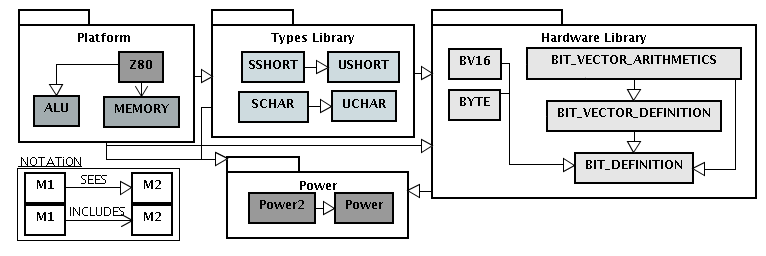
\includegraphics[width=.77\textwidth]{diagramaEstrutural_vertical_ProB.png}
 \caption{Dependency diagram of the Z80 model.}
\label{fig:hardware-definition-graph}
\end{figure}

\subsection{Bit representation and manipulation}
\label{subsec:HardwareLibrary1}

The entities defined in the module $\textit{BIT\_DEFINITION}$ are the
type for bits, logical operations on bits (negation, conjunction,
disjunction, exclusive disjunction), and a conversion function from
Booleans to bits.

We model bits as a set of integers: $\textit{BIT} =
\textit{0..1}$. The negation is an unary function on bits and it is
defined as:
$$
\begin{array}{l}
\textit{bit\_not}  \in  \textit{BIT}  \fun  \textit{BIT}  \land 
\textit{bit\_not} \rm = \rm \{ \rm 0  \mapsto  \rm 1 , \rm 1  \mapsto  \rm 0 \rm \}
\end{array}
$$
%\forall ( \textit{bb}). (\textit{bb} \in \textit{BIT} \implies {bit\_not}(\textit{bb}) =1-\textit{bb})\\

The module also provides lemmas on negation that may be useful for the
users of the library to develop proofs:
$$
\begin{array}{l}
%  \textit{bit\_not}(0) = 1;  \textit{bit\_not}(1) = 0; \\
\forall (\textit{bb}).(\textit{bb} \in \textit{BIT} \implies \textit{bit\_not}(\textit{bit\_not}(\textit{bb})) = \textit{bb})
\end{array}
$$
Conjunction is a binary function on bits and it is defined as:
$$
\begin{array}{l}
\textit{bit\_and} \in \textit{BIT} \times \textit{BIT} \fun \textit{BIT} \land \\
\forall (\textit{b1}, \textit{b2}).(\textit{b1}  \in \textit{BIT}  \land \textit{b2} \in \textit{BIT} \implies \\
\quad ((\textit{bit\_and}(\textit{b1}, \textit{b2}) = 1) \iff (\textit{b1} = 1)  \land  (\textit{b2} = 1)))
\end{array}
$$
The module provides the following lemmas for commutativity and associativity:
$$
\begin{array}{l}
%  \textit{bit\_and}(0,0) = 0;  \textit{bit\_and}(0,1) = 0; \\
%  \textit{bit\_and}(1,0) = 0;  \textit{bit\_and}(1,1) = 1; \\
\forall (\textit{b1},\textit{b2}).(\textit{b1} \in \textit{BIT} \land \textit{b2} \in \textit{BIT} \implies \\
\quad (\textit{bit\_and}(\textit{b1}, \textit{b2}) = \textit{bit\_and}(\textit{b2},\textit{b1})))\land \\
\forall (\textit{b1},\textit{b2},\textit{b3}).(\textit{b1} \in \textit{BIT} \land  \textit{b2} \in \textit{BIT} \land \textit{b3} \in \textit{BIT} \implies \\
\quad (\textit{bit\_and}(\textit{b1}, \textit{bit\_and}(\textit{b2},\textit{b3})) = \textit{bit\_and}(\textit{bit\_and}(\textit{b1},\textit{b2}),\textit{b3})))\\
% \forall (\textit{b1}).(\textit{b1} \in \textit{BIT} \implies (\textit{bit\_and}(\textit{b1}, 1) = \textit{b1})); \\
% \forall (\textit{b1}).(\textit{b1} \in \textit{BIT} \implies (\textit{bit\_and}(\textit{b1}, 0) = 0));
\end{array}
$$
The module provides definitions of $\textit{bit\_or}$ (disjunction)
and $\textit{bit\_xor}$ (exclusive disjunction), as well as lemmas on
those operators. These are standard and their expression in B is
similar to $\textit{bit\_and}$.

Finally, the conversion from Boolean to bit is simply defined as:
$$
\begin{array}{l}
\textit{bool\_to\_bit} \in \BOOL \fun \textit{BIT} \land \textit{bool\_to\_bit} = \{ \TRUE \mapsto 1, \FALSE \mapsto 0 \} \\
\end{array}
$$
All the lemmas that are provided in this module have been
automatically proved by the prover of Atelier-B.


\subsection{Representation and manipulation of bit vectors}
\label{subsec:HardwareLibrary2}

Sequences are predefined objects in B and are natural candidates to
represent bit vectors. In B, sequences are functions whose domain
is an integer range with lower bound 1 (one). Indices in bit vectors
usually range from 0 (zero) upwards and the model we propose obeys
this convention by making an offset where necessary, so that
predefined functions and proof rules may be used. We define bit
vectors as non-empty sequences of bits: $\textit{BIT\_VECTOR} =
\seq1 (\textit{BIT})$. As $\textit{BIT\_VECTOR}$ is an infinite set,
this definition hinders the animation in ProB.  As a workaround, we
defined specialized types \textit{BYTE} and \textit{BV16} without
reference to \textit{BIT\_VECTOR}.

% CAN COMMENT TO REDUCE SPACE
%The function $\textit{bv\_size}$ returns the size of a given bit vector. It is basically a wrapper for the
%predefined function $\textbf{size}$ that applies to sequences.
%
%$
%\begin{array}{l}
%\textit{bv\_size} \in \textit{BIT\_VECTOR} \fun \nat_1 \land \\
%\textit{bv\_size} = \lambda bv . (bv \in \textit{BIT\_VECTOR} \mid \textbf{size}(bv))
%\end{array}
%$

We also define two functions $\textit{bv\_set}$ and
$\textit{bv\_clear}$ that, given a bit vector, and a position in a
bit vector, returns the bit vector resulting from setting the
corresponding position to 1 and 0, and a function $\textit{bv\_get}$
that, given a bit vector and a valid position, returns the value of
the bit at that position. Only the first definition is shown here:
$$
\begin{array}{l}
\textit{bv\_set} \in \textit{BIT\_VECTOR} \times \nat \fun \textit{BIT\_VECTOR} \land \\ \textit{bv\_set} =
\lambda v, n . (v \in \textit{BIT\_VECTOR} \land n \in \nat \land n <\textit{size}(v)
\mid v \lover \{ n+1 \mapsto 1 \})
\end{array}
$$

Function $bv\_catenate$ takes as parameters two bit vectors $v$ and
$w$, and returns the concatenation of $v$ and $w$, such
that $v$ constitutes the most significant part of the result.


% $
% \begin{array}{l}
% \textit{bv\_catenate} \in \textit{BIT\_VECTOR} \times \textit{BIT\_VECTOR} \fun \textit{BIT\_VECTOR} \land \\
% \textit{bv\_catenate} = \lambda v, w \bullet (v \in \textit{ BIT\_VECTOR} \land w \in \textit{ BIT\_VECTOR}  \mid v 
% %\conc
%   w)
% \end{array}
% $


\hspace*{0.00in} \it bv\_catenate  $\in$  \it BIT\_VECTOR  $\times$  \it BIT\_VECTOR  $\fun$ \it
BIT\_VECTOR $\land$\\
\hspace*{0.21in} \it bv\_catenate \rm =  $\lambda$  v\rm ,\it w \rm . \rm (\it v 
$\in$  \it BIT\_VECTOR $\land$ \it w $\in$  \it BIT\_VECTOR  $\mid$  \it v\^ \it w\rm ) %$\cat$

%COMMENT TO REDUCE SPACE
%We also define a function $\textit{bv\_zero}$ that, given a positive
%integer $n$, return a bit vector of size $n$, with all bits set to 0.
%A similar function, called $\textit{bv\_one}$, with all bits set to 1
%is also defined but not presented here.
%
%$
%\begin{array}{l}
%\textit{bv\_zero} \in \nat_1 \fun \textit{BIT\_VECTOR} \land \\
%\textit{bv\_zero} = \lambda n . (n \in \nat_1 \mid 1..n \times \{0\}) 
%\end{array}
%$
%


Additionally, the module provides definitions for the classical
logical combinations of bit vectors: $\textit{bit\_not}$,
$\textit{bit\_and}$, $\textit{bit\_or}$ and $\textit{bit\_xor}$. Only
the first two are presented here. The domain of the binary operators
is restricted to pairs of bit vectors of the same length:
$$
\begin{array}{l}
\textit{bv\_not} \in \textit{BIT\_VECTOR} \fun \textit{BIT\_VECTOR} \land \\
\textit{bv\_not} = \lambda v . (v \in \textit{BIT\_VECTOR} \mid \quad \lambda i . (1 .. \textit{size}(v)) \mid \textit{bit\_not}(v(i))) \land \\
\textit{bv\_and} \in \textit{BIT\_VECTOR} \times \textit{BIT\_VECTOR} \fun \textit{BIT\_VECTOR} \land \\
\textit{bv\_and} = \lambda v_1, v_2 . (v_1 \in \textit{BIT\_VECTOR} \land v_2 \in \textit{BIT\_VECTOR} \land \\
\textit{size}(v_1) = \textit{size}(v_2) \mid \lambda i . (1 .. \textit{size}(v_1)) \mid
\textit{bit\_and}(v_1(i), v_2(i)))
\end{array}
$$
We provide several lemmas on bit vector operations. These lemmas
express properties on the size of the result of the operations
as well as classical algebraic properties such as associativity
and commutativity.

\subsection{Modeling bytes and bit vectors of length 16}
\label{subsec:HardwareLibrary3}

Bytes, i.e. bit vectors of length 8, are a common entity in hardware
design. We provide the following definitions:

\hspace*{0.0in}\it BYTE\_WIDTH \rm = 8 $\land$ \it BYTE\_INDEX \rm = 1 $\upto$ \rm  BYTE\_WIDTH\rm  \hspace*{0.03in} $\land$

\hspace*{0.0in}\it PHYS\_BYTE\_INDEX \rm = \rm 0 $\upto$ \rm (\it BYTE\_WIDTH\rm -\rm 1\rm )\hspace*{0.03in} $\land$ \hspace*{0.0in}\it BYTE \rm =\rm (\it BYTE\_INDEX  $\fun$  \it BIT\rm )\hspace*{0.0in} $\land$  


\hspace*{0.0in}$\forall$ \rm (\it b1\rm )\rm .\rm (\it b1  $\in$  \it BYTE  $\implies$  \bf size\rm (\it b1\rm )\rm =\it BYTE\_WIDTH  $\land$  \it b1  $\in$  \bf seq1\rm (\it BIT\rm )\rm ) 

%\hspace*{0.0in}\it BYTE \rm = \rm \{ \it bt  $\mid$  \it bt $\in$ \it BIT\_VECTOR  $\land$  \it size\rm (\it bt\rm )\rm =\it BYTE\_WIDTH\rm \} $\land$

%\hspace*{0.0in}\it BYTE\_ZERO  $\in$  \it BYTE  $\land$ \it BYTE\_ZERO \rm = \it BYTE\_INDEX  $\times$  \rm \{\rm 0\rm \}

$\textit{BYTE\_INDEX}$ is the domain of the functions modeling
bytes. It starts at 1 to be compatible with sequences. However, since
the hardware community starts indexing from zero, definition
$\textit{PHYS\_BYTE\_INDEX}$ provides functionalities obeying this
convention. Type $\textit{BYTE}$ is as a specialized type of
$\textit{BIT\_VECTOR}$, with a size constraint. Other specific
definitions are provided to facilitate further modeling: the type
$\textit{BV16}$ is created for bit vectors of length 16 in a similar
way.

\subsection{Bit vector arithmetic}
\label{subsec:Types}
 

Bit vectors are used to represent and combine numbers: integer ranges
(signed or unsigned). Therefore, our library includes functions to
manipulate such data, for example, the function $\textit{bv\_to\_nat}$
maps bit vectors to natural numbers:
$$
\begin{array}{l}
\textit{bv\_to\_nat} \in \textit{BIT\_VECTOR} \fun \nat  \land \\
\textit{bv\_to\_nat} = \lambda v .  (v \in \textit{BIT\_VECTOR} \mid  \sum i . (i \in \dom(v) . v(i)
\times 2^{i-1}))
\end{array}
$$

An important lemma associated to this definition is: 
$$\forall n . (n \in \nat_1 \implies \textit{bv\_to\_nat}(\textit{nat\_to\_bv}(n)) = n).$$



\subsection{Basic data types}

The definition of instruction sets usually have bit vector and integer
types as listed in table~\ref{tab:types}. For each type, a number of
functions are defined, including conversion between different types.

\begin{table}[h]
\caption{Details of basic data types}
\label{tab:types}
\begin{center}
\begin{tabular}{|c|c|c|c|c|}
\hline
 \textit{Type\ Name} & \textit{Range} & \textit{Physical Size}  & \textit{Num. POs} & \textit{Library} \\\hline
 BIT & 0..1 & 1 bit &   118 & Hardware \\\hline 
 BYTE & -- & 1 bytes &  154 & Hardware \\\hline
 BV16 & -- & 2 bytes &  75 & Hardware \\ \hline
 UCHAR & 0..255 & 1 byte &  30 & Types \\\hline
 SCHAR & -128..127 & 1 byte & 30 & Types \\\hline 
 USHORT & 0..65535 & 2 byte & 62 & Types \\\hline
 SSHORT & -32768..32767 & 2 bytes & 62 & Types \\\hline 
\end{tabular}
\end{center}
\end{table}

Usually, each type module just needs to specialize definitions that
are given in the hardware modeling library.  For example, the function
$\textit{bv\_to\_nat}$ from bit vector arithmetic is specialized to
$\textit{byte\_uchar}$. As the set $\textit{BYTE}$ is a subset of the
$\textit{BIT\_VECTOR}$, this function can be defined as follows:
$$
\begin{array}{l}
\textit{byte\_uchar} \in \textit{BYTE} \fun \nat \land \\
\textit{byte\_uchar} = \lambda (v) . ( v \in BYTE | bv\_to\_nat(v) )
\end{array}
$$

The definitions of the library types reuse the basic definitions from
the hardware library. This provides greater confidence and facilitates
the proof process, because the prover can reuse the previously defined
lemmas.


%The inverse function $\textit{uchar\_byte}$ is easily defined:
%
%$
%\begin{array}{l}
%\textit{uchar\_byte} \in \textit{UCHAR}  \fun  \textit{BYTE}  \land \\
%   \textit{uchar\_byte} = \ (\textit{byte\_uchar}) ^{-1}
%\end{array}
%$

We also created lemmas on pairs of dual conversion functions, such as:
$$
 \begin{array}{l}
  \forall (val) . (val \in \textit{UCHAR} |
  \textit{byte\_uchar}(\textit{uchar\_byte}(val)) = val) \land\\
  \forall (by) . (by \in \textit{BYTE} |
  \textit{uchar\_byte}(\textit{byte\_uchar}(by)) = by)
 \end{array}
$$

%TODO:[NEW PARAGRAPH-TO-REVIEW]
Similarly, several other general functions and lemmas were created for all other data types.
Some times, we need  create arithmetic and logic functions that are more specific for a
determined microprocessor, like Z80 that is presented in the section \ref{sec:z80}. 

%TODO:[NEW PARAGRAPH-TO-REVIEW]
The definitions, functions and properties from hardware library and types library are difficult to verify,
on the other hand  these libraries can be reused in several others  microprocessors without to verify again.
Nearly 50\% of all these proof obligations shown in the Table~\ref{tab:types} are verified automatically 
or with few user pass\footnote{The user pass are steps that aid the prover to find the proof.} .
But many others proof obligations are difficult to verify, because they involve functions
that contain arithmetic expressions that are complex to manipulate with the interactive
prover of AtelierB.  However, all theses 531 proof obligations were verified completely.


\subsection{Verification of hardware library and types library} 
\label{sec:VerificationHardwareLibrary}

This section presents the verification of the aforementioned modules
using AtelierB provers.  By default, AtelierB~\cite{atelierB} does not
generate proof obligations to check the type of functions defined in
the $PROPERTIES$ clause of a machine. For example, the definition $inc
\in \{0,1\} \fun \{0,1\} \land inc = \lambda(x).( x \in \{0,1\} | x +
1)$, does not create a proof obligation to check the consistency of
the definition. However, this definition is inconsistent since
$inc(1)=2$ and $ 2 \not\in \{0,1\}$.

To avoid such inconsistencies, we state separately the required
properties in the \textit{ASSERTIONS\/} clause: this causes
corresponding proof obligations to be generated and verified. However,
we have not been able to build the corresponding proofs using the 
rule base included in the free distribution of AtelierB. So we
formalized new proof rules to check these properties in AtelierB and
used them in the interactive prover of AtelierB.

The hardware library has many conversion functions with
arithmetic,  for example, Bit\_vector to Natural, Natural to
Bit\_vector, Integer to Bit\_vector and Bit\_vector to Integer. These
functions are organized in modules and each module contains auxiliary
functions for a data type. The modules are represented by gray
rectangles in Figure \ref{DiagramTypesRules}.

\begin{figure}[he]
\centering
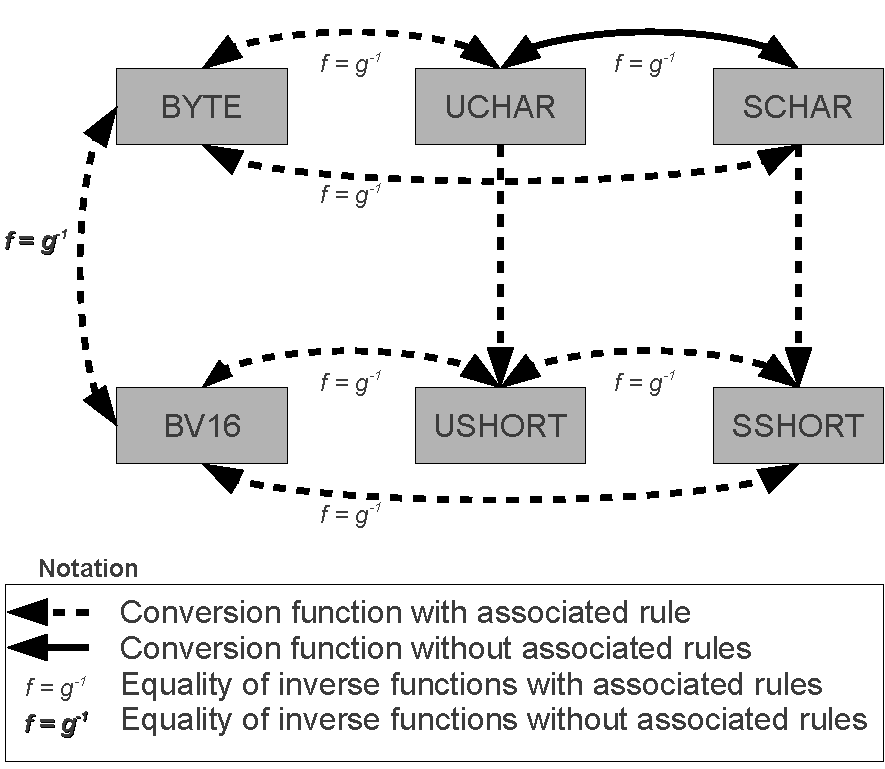
\includegraphics[width=3.in]{images/Diagram_Types_and_Rules.pdf}
\caption{Conversion functions}
\label{DiagramTypesRules}
\end{figure}


The conversion functions need to satisfy two properties: bijectivity
and equality to the reverse of the dual conversion function. Three
such proof obligations were verified automatically with AtelierB: (\it
uchar\_schar\rm \ $\in$ \textit{UCHAR} $\bij$ \textit{SCHAR}), (\it
schar\_uchar\rm \ $\in$ \textit{SCHAR} $\bij$ \textit{UCHAR}) and (\it
byte\_bv16\rm \ $=$ \it bv16\_byte\rm $^{-1}$).
%\begin{enumerate}
%
%\item (\it uchar\_schar\rm \ $\in$ \textit{UCHAR} $\bij$ \textit{SCHAR})
%\item (\it schar\_uchar\rm \ $\in$ \textit{SCHAR} $\bij$ \textit{UCHAR})
%\item (\it byte\_bv16\rm \ $=$ \it bv16\_byte\rm $^{-1}$) 
%
%\end{enumerate}
For the remaining proof obligations, we again had to create new proof
rules. There are three kinds of proof rules, that we illustrate by giving
one example each:

%Four conditions are needed to be a bijective function:
%
%\begin{description}
%\item $func$ is a function:\\
%$\forall$ \rm (\it xx\rm ,\it yy\rm ,\it zz\rm )\rm .\rm ( \it xx  $\in$  \bf dom\rm (\it func\rm )  $\land$  \it yy $\in$  \bf ran\rm (\it func\rm )  $\land$ \\ \it zz $\in$  \bf ran\rm (\it func\rm )  $\land$ \rm ( \it xx $\mapsto$  \it yy\rm )  $\in$  \it func  $\land$  \rm ( \it xx $\mapsto$  \it zz\rm )  $\in$  \it func  $\implies$  \it yy\rm =\it zz \rm )
%
%\item $func$ is an injective function:\\
%$\forall$ \rm (\it vv\rm ,\it xx\rm )\rm .\rm ( \it vv $\in$  \bf dom\rm (\it func\rm )  $\land$  \it xx  $\in$  \bf dom\rm (\it func\rm )  $\implies$  \it func\rm (\it vv\rm )\rm =\it func\rm (\it xx\rm ) \rm )
%
%\item $func$ is a total function:\\
%$\forall$ \it xx\rm .\rm ( \it xx  $\in$  \bf dom\rm (\it func\rm )  $\implies$   $\exists$ \it yy\rm .\rm ( \it yy  $\in$  \bf ran\rm (\it func\rm )  $\land$  \it func\rm (\it xx\rm )\rm =\it yy \rm )\rm ) 
%
%\item $func$ is surjective function:\\
% $\forall$ \it yy\rm .\rm ( \it yy $\in$  \bf ran\rm (\it func\rm ) $\implies$   $\exists$ \it xx\rm .\rm ( \it xx  $\in$  \bf dom\rm (\it func\rm ) $\land$  \it func\rm (\it xx\rm )\rm =\it yy \rm )\rm ) 
%
%
%\end{description} 
%
%Here, two conversion functions between bit vectors and the natural are presented. These functions are finite and convert from \textit{BYTE} to \textit{UCHAR} and vice versa.\textit{UCHAR} is a range between 0 and 255 and \textit{BYTE} is a bit vector with eight elements enumerated starting from 1. We need to prove that $byte\_uchar$  and $uchar\_byte$  are bijective functions and  $byte\_uchar = uchar\_byte^{-1}$. These functions are defined as follows:
%\begin{description}
%
%
%\item\it byte\_uchar \rm = $\lambda$  \rm ( \it v0 \rm ) \rm . \rm ( \it v0  $\in$  \it BYTE  $\mid$ \hspace*{0.10in}\it 2$^{7}$ $\times$ \it v0\rm (\rm 8\rm )\rm +\it 2$^{6}$  $\times$ \it v0\rm (\rm 7\rm )\rm + \it 2$^{5}$ $\times$ \it v0\rm (\rm 6\rm )\rm +\it 2$^{4}$ $\times$ \it v0\rm (\rm 5\rm ) \rm + \it 2$^{3}$  $\times$  \it v0\rm (\rm 4 \rm ) \rm + \it 2$^{2}$  $\times$ \it v0\rm (\rm 3\rm ) \rm + \it 2$^{1}$  $\times$  \it v0\rm (\rm 2\rm ) \rm + \it 2$^{0}$  $\times$  \it v0\rm (\rm 1\rm )\rm) 
%
%\item\it uchar\_byte \rm = $\lambda$  \rm ( \it v0 \rm ) \rm . \rm ( \it v0  $\in$  \it UCHAR $\mid$ \rm [\rm (\it v0   $\mod$ \it 2$^{1}$\rm ) $\div$ \it 2$^{0}$\rm , \rm (\it v0  $\mod$  \it 2$^{2}$\rm ) $\div$ \it 2$^{1}$\rm , \rm (\it v0  $\mod$  \it 2$^{3}$\rm ) $\div$ \it 2$^{2}$\rm , \rm (\it v0  $\mod$  \it 2$^{4}$\rm ) $\div$ \it 2$^{3}$\rm , \rm (\it v0  $\mod$  \it 2$^{5}$\rm ) $\div$ \it 2$^{4}$\rm , \rm(\it v0  $\mod$  \it 2$^{6}$\rm ) $\div$ \it 2$^{5}$\rm ,\rm (\it v0  $\mod$  \it 2$^{7}$\rm ) $\div$ \it 2$^{6}$\rm , \rm (\it v0  $\mod$  \it 2$^{8}$\rm ) $\div$ \it 2$^{7}$\rm \rm ] \rm)
%
%\end{description}
%
%The equivalent definitions using B sequence notation and set notation are:\\
%\it uchar\_byte \rm = \rm \{ \rm 0 $\mapsto$ \rm \rm [\rm 0\rm ,\rm 0\rm ,\rm 0\rm ,\rm 0\rm ,\rm 0\rm ,\rm 0\rm ,\rm 0\rm ,\rm 0\rm \rm ]\rm, \ldots  , \rm 2\rm 5\rm 5 $\mapsto$ \rm \rm [\rm 1\rm ,\rm 1\rm ,\rm 1\rm ,\rm 1\rm ,\rm 1\rm ,\rm 1\rm ,\rm 1\rm ,\rm 1\rm \rm ]\rm \}  \\
%\it byte\_uchar \rm =  \rm \{\rm \rm [\rm 0\rm ,\rm 0\rm ,\rm 0\rm ,\rm 0\rm ,\rm 0\rm ,\rm 0\rm ,\rm 0\rm ,\rm 0\rm \rm ] $\mapsto$ \rm 0\rm, \ldots , \rm \rm [\rm 1\rm ,\rm 1\rm ,\rm 1\rm ,\rm 1\rm ,\rm 1\rm ,\rm 1\rm ,\rm 1\rm ,\rm 1\rm \rm ] $\mapsto$ \rm 2\rm 5\rm 5 \rm \} \rm 
%
%\paragraph{B Rules:}
%These rules represent that  $byte\_uchar$  and $uchar\_byte$  are bijective functions and  $byte\_uchar = uchar\_byte^{-1}$. These rules are used on interactive prover of Atelierb.



\begin{enumerate}

\item For the proof obligation (\it byte\_uchar\rm \ $\in$ \textit{BYTE} $\bij$
\textit{UCHAR}), the proof rule is:\\
$\lambda$ \it v0\rm .\rm (\it v0 $\in$  \rm 1 $\upto$ \rm 8  $\fun$  \rm \{\rm 0\rm ,\rm 1\rm \}  $\mid$  \rm 1\rm 2\rm 8 $\times$ \it v0\rm (\rm 8\rm )\rm +\rm 6\rm 4 $\times$ \it v0\rm (\rm 7\rm )\rm +\rm 3\rm 2 $\times$ \it v0\rm (\rm 6\rm )\rm +\rm 1\rm 6 $\times$ \it v0\rm (\rm 5\rm )\rm +\rm 8 $\times$ \it v0\rm (\rm 4\rm )\rm +\rm 4 $\times$ \it v0\rm (\rm 3\rm )\rm +\rm 2 $\times$ \it v0\rm (\rm 2\rm )\rm +\rm 1 $\times$ \it v0\rm (\rm 1\rm )\rm ) \rm $\in$ \rm (\rm 1 $\upto$ \rm 8  $\fun$  \rm \{\rm 0\rm ,\rm 1\rm \}\rm )  $\bij$  \rm 0 $\upto$ \rm 2\rm 5\rm 5 \\

\item For the proof obligation (\it uchar\_byte\rm \ $\in$ \textit{UCHAR} $\bij$
\textit{BYTE}), the proof rule is:\\ $\lambda$ \it v0\rm .\rm (\it v0 $\in$  \rm 0$\upto$255  $\mid$  \rm \rm  [(\it v0  $\mod$  \rm 2)$\div$1,(\it v0  $\mod$  \rm 4)$\div$\rm 2\rm,(\it v0  $\mod$  \rm 8)$\div$\rm 4\rm,(\it v0  $\mod$  \rm 16)$\div$\rm 8\rm,(\it v0  $\mod$  \rm 32)$\div$\rm 1\rm 6\rm,(\it v0  $\mod$  \rm 6\rm 4)$\div$\rm 3\rm 2\rm,(\it v0  $\mod$  \rm 1\rm 2\rm 8)$\div$\rm 6\rm 4\rm,(\it v0  $\mod$  \rm 2\rm 5\rm 6)$\div$\rm 1\rm 2\rm 8\rm \rm ]\rm ) \rm   $\in$  \rm 0 $\upto$ \rm 2\rm 5\rm 5   $\bij$ \rm (\rm 1 $\upto$ \rm 8  $\fun$  \rm \{\rm 0\rm ,\rm 1\rm \}\rm )\\


\item For the proof obligation (\it byte\_uchar\rm  =  \it
uchar\_byte\rm$^{-1}$), the proof rule is:\\ $\lambda$ \it v0\rm .\rm (\it v0 $\in$  \rm 1 $\upto$ \rm 8  $\fun$  \rm \{\rm 0\rm ,\rm 1\rm \}  $\mid$  \rm 1\rm 2\rm 8 $\times$ \it v0\rm (\rm 8\rm )\rm +\rm 6\rm 4 $\times$ \it v0\rm (\rm 7\rm )\rm +\rm 3\rm 2 $\times$ \it v0\rm (\rm 6\rm )\rm +\rm 1\rm 6 $\times$ \it v0\rm (\rm 5\rm )\rm +\rm 8 $\times$ \it v0\rm (\rm 4\rm )\rm +\rm 4 $\times$ \it v0\rm (\rm 3\rm )\rm +\rm 2 $\times$ \it v0\rm (\rm 2\rm )\rm +\rm 1 $\times$ \it v0\rm (\rm 1\rm )\rm )=($\lambda$ \it v0\rm .\rm (\it v0 $\in$  \rm 0$\upto$255  $\mid$  \rm \rm  [(\it v0  $\mod$  \rm 2)$\div$1,(\it v0  $\mod$  \rm 4)$\div$\rm 2\rm,(\it v0  $\mod$ \rm 8) $\div$\rm 4\rm,(\it v0  $\mod$  \rm 16)$\div$\rm 8\rm,(\it v0  $\mod$  \rm 32)$\div$\rm 1\rm 6\rm,(\it v0  $\mod$ \rm 6\rm 4)$\div$\rm 3\rm 2\rm,(\it v0  $\mod$  \rm 1\rm 2\rm 8)$\div$\rm 6\rm 4\rm,(\it v0  $\mod$  \rm 2\rm 5\rm 6)$\div$\rm 1\rm 2\rm 8\rm \rm ]\rm )\rm)$^{-1}$
\end{enumerate}

Eight proof obligations require that conversion functions are finite. %: \it
% byte\_uchar $\in$ $\finset$\rm (\it byte\_uchar\rm ); \it uchar\_byte  $\in$
% $\finset$\rm (\it uchar\_byte\rm ); \it ushort\_bv16 $ \in \finset$\rm (\it
% ushort\_bv16\rm ); \it bv16\_ushort $ \in \finset$\rm (\it bv16\_ushort\rm ); \it
% byte\_schar $ \in \finset$\rm (\it byte\_schar\rm ); \it schar\_byte $ \in
% \finset$\rm (\it schar\_byte\rm ); \it sshort\_bv16 $ \in \finset$\rm (\it
% sshort\_bv16\rm ); and \it bv16\_sshort $ \in \finset$\rm (\it bv16\_sshort\rm).
 These proof obligations were verified using the expression evaluator of ProB.
Finally, we have included rules related to binary arithmetic as developed
in~\cite{Leibnizens}. These rules are used in the interactive theorem prover with
binary arithmetic to prove important properties~\cite{James2010,Dasgupta2006}.



\section{A B model of the Z80 instruction set}
\label{sec:z80}

The \textit{Z80} is a CISC microcontroller developed by
\textit{Zilog}~\cite{Z80_manual}. The Z80 is composed by different
elements and a simplified internal organization is shown in the Figure
\ref{fig:DiagramBlock}.  This figure has some important elements of
Z80 CPU: ALU, registers of 8 and 16 bits and input/output ports.

\begin{figure}[h] \centering
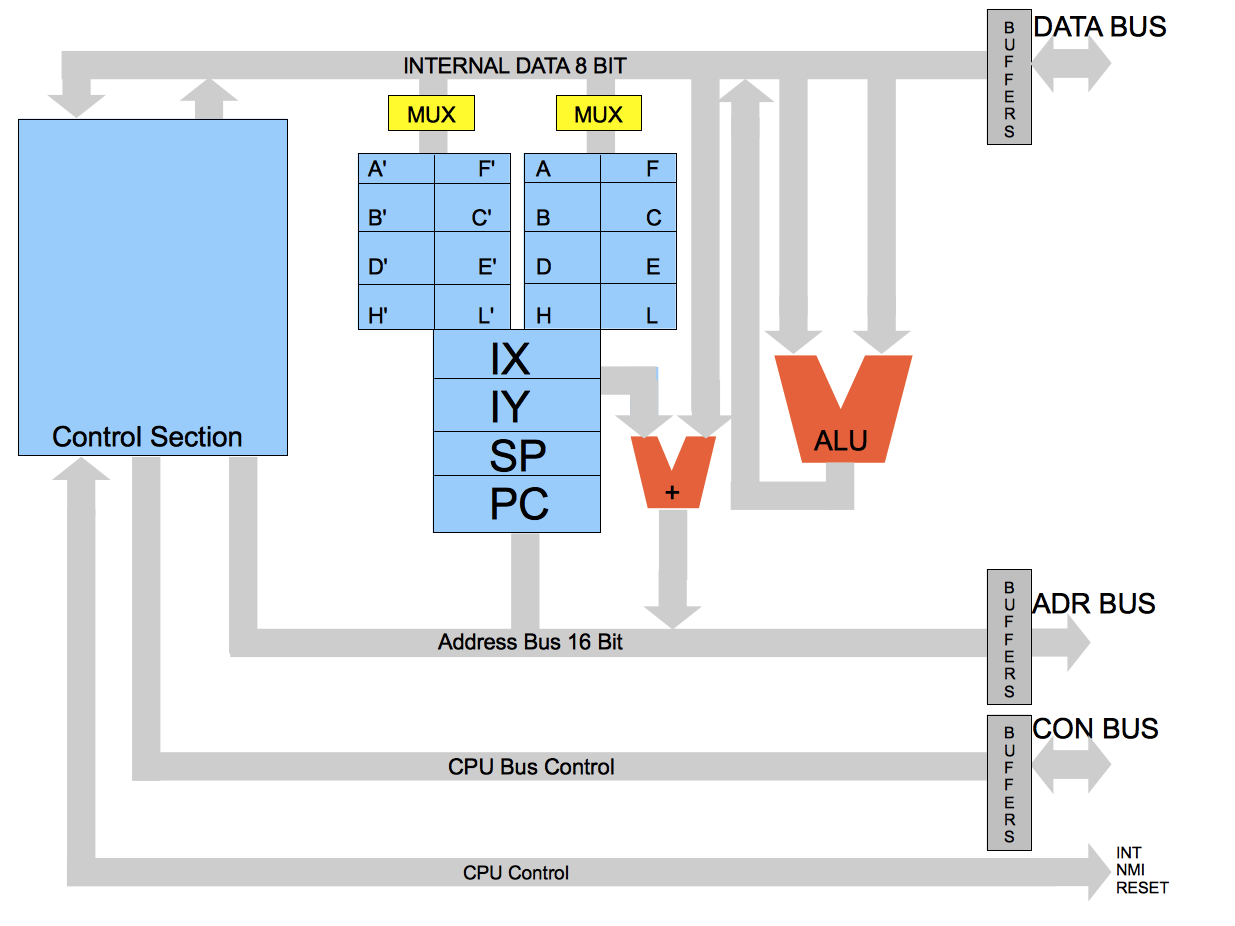
\includegraphics[width=0.70\textwidth]{images/Architecture.png}
\caption{Simplified internal organization of Z80 CPU.}
\label{fig:DiagramBlock}
\end{figure}


The Z80 has 158 different instructions, including all the 78 from the Intel 8080
microprocessor, and all of them were formally specified in B. These instructions are classified
into these categories: load and exchange; block transfer and search; arithmetic
and logical; rotate and shift; bit manipulation; jump, call and return;
input/output; and basic cpu control. Each category of instruction has different
elements of specification.


This section shows the elements that make up the different types of
instructions. The main elements are specified in the microcontroller module Z80
and parts of it are presented below.  Basically, the state of microcontroller is
formed by data from program counter, ports, registers, etc. The transitions
between the states are actioned by execution of instruction or an external
action. Groups of registers are represented by the variables of the
specification states that appear in clause \textit{VARIABLES}. The declaration
of valid states of variables is in the \textit{INVARIANT} clause and the initial
state is defined in the \textit{INITIALISATION} clause. The assembly
instructions are defined by the clause \textit{OPERATIONS} and, in general, each
instruction has three actions: update the program counter, update the flag
register and its main effect.
% Several functions were created to Z80.
General functions that can be used in other microcontroller models are defined
in the modules of data types. Specific functions of the microcontroller are
defined in the ALU (arithmetic logic unit) module.



The main module includes an instance of the memory module and accesses the
definitions from basic data types modules and the \textit{ALU} module.

	\begin{center}
	\begin{sloppypar}
	
	  \begin{tabbing}
	    \begin{array}[t]{l}
		\bf MACHINE\\
		\hspace*{0.15in}\it Z80\\
		\bf INCLUDES\\
		\hspace*{0.10in}\it MEMORY
	    \end{array}
	     \hspace*{1cm} 
	    \begin{array}[t]{l}
	    \bf SEES\\
		\hspace*{0.10in}\it ALU, \it BIT\_DEFINITION, \it BIT\_VECTOR\_DEFINITION,\\
		\hspace*{0.10in}\it BYTE\_DEFINITION, \it BV16\_DEFINITION,\\
		\hspace*{0.10in}\it UCHAR\_DEFINITION, \it SCHAR\_DEFINITION,\\
		\hspace*{0.10in}\it SSHORT\_DEFINITION ,\it USHORT\_DEFINITION\\
	    \end{array}
	  \end{tabbing}
	  
	 \end{sloppypar} 
	\end{center}


\subsection{Modeling registers}

The Z80 CPU includes alternative set of accumulator, flag and general registers.
The CPU contains a stack pointer ($\textit{sp}$), program counter
($\textit{pc}$), two index registers ($\textit{ix}$ and $\textit{iy}$), an
interrupt register ($\textit{i\_}$), a refresh register ($\textit{r\_}$), two
bits ($\textit{iff1}$, $\textit{iff2}$) used to control the interruptions, a
pair of bits to define the interruption mode ($\textit{im}$) and the input and
output ports ($\textit{i\_o\_ports}$). These definitions are represented by
\textit{INVARIANT}.
  

\begin{sloppypar}
\bf INVARIANT

\hspace*{0.10in}\it rgs8  $\in$  \it id\_reg\_8  $\fun$  \it BYTE  $\land$ \it pc  $\in$  \it INSTRUCTION  $\land$  \it sp  $\in$  \it BV16 $\land$  \it ix  $\in$  \it BV16  $\land$

\hspace*{0.10in}\it iy  $\in$  \it BV16  $\land$ \it i\_  $\in$  \it BYTE  $\land$  \it r\_ $\in$  \it BYTE  $\land$ \it iff1  $\in$  \it BIT  $\land$ \it iff2  $\in$  \it BIT  $\land$ 

\hspace*{0.10in}\it im $\in$ (\it BIT $\times$ \it BIT\rm )  $\land$  \it i\_o\_ports  $\in$  \it BYTE  $\fun$  \it BYTE
\end{sloppypar}


 

% Features of microcontroller
The internal registers contains 176 bits of read/write memory that are
represented by identifiers used as parameters in the instructions . It includes
two sets of six general purpose registers which may be used individually as
8-bit registers or as 16-bit register pairs.  The working registers are
represented by variable $\textit{rgs8}$. The domain of $\textit{rgs8}$
($\textit{id\_reg8}$) is a set formed by identifiers of registers of 8 bits.
These registers are called main register set (\textit{a0,b0,c0,d0,e0,f0,h0,l0})
and alternate register set (\textit{a\_0,b\_0,c\_0,d\_0,e\_0,f\_0,h\_0,l\_0}).
These registers can be accessed in pairs, forming 16-bits, resulting in another
set of identifiers of 16-bits registers, named $\textit{id\_reg16}$. These sets
are represented below.

\begin{sloppypar}

	\bf SETS\\
\hspace*{0.10in}\it id\_reg\_8 \rm = \rm \{ \it a0\rm, \it f0\rm, \it b0\rm, \it
c0\rm, \it d0\rm, \it e0\rm, \it h0\rm, \it l0\rm, \it a\_0\rm,  \it f\_0\rm,
\it b\_0\rm, \it c\_0\rm, \it d\_0\rm, \it e\_0\rm, \it h\_0\rm, \it l\_0 \rm
\};\\ \hspace*{0.10in}\it id\_reg\_16 \rm = \rm \{  \it AF \rm, \it BC\rm, \it
DE\rm, \it HL\rm, \it SP\rm\}
	

\end{sloppypar}

%\begin{sloppypar}
%
%	\bf SETS\\
%	\hspace*{0.10in}\it id\_reg\_8 \rm = \rm \{ \it a0 \rm , \it f0 \rm , \it f\_0 \rm , \it a\_0 \rm ,\\
%	\hspace*{0.93in}\it b0 \rm , \it c0 \rm , \it b\_0 \rm , \it c\_0\rm,\\
%	\hspace*{0.93in}\it d0 \rm , \it e0 \rm , \it d\_0 \rm , \it e\_0\rm,\\
%	\hspace*{0.93in}\it h0 \rm , \it l0 \rm , \it h\_0 \rm , \it l\_0\};\\
%	\hspace*{0.10in}\it id\_reg\_16 \rm = \rm \{ \it BC \rm , \it DE \rm , \it HL \rm , \it SP \rm , \it AF \rm \}
%\end{sloppypar}


The main working register of Z80 is the accumulator ($\textit{rgs8(a0)}$) used for arithmetic/logic, input/output and loading/storing operations.
Another important element is the ``f'' register ($\textit{rgs8(f0)}$),  that is
used as a \textbf{flag register}. This register uses only six bits to represent the execution result status of each instruction.
According to the official manual the bits 3 and 5 are not used and the others bits have the follow meaning: %$\textit{bv\_get(rgs8(f0),0)}$ - the carry bit; $\textit{bv\_get(rgs8(f0),1)}$ - the add/subtract bit; $\textit{bv\_get(rgs8(f0),2)}$ - the parity or overflow bit; $\textit{bv\_get(rgs8(f0),4)}$ - the half carry bit; $\textit{bv\_get(rgs8(f0),6)}$ - the zero bit; and $\textit{bv\_get(rgs8(f0),7)}$ - the sign bit.
\begin{description}
  \item[$\textit{bv\_get(rgs8(f0),0)}$] - The Carry bit.
  \item[$\textit{bv\_get(rgs8(f0),1)}$] - The Add/Subtract bit.
  \item[$\textit{bv\_get(rgs8(f0),2)}$] - The Parity or Overflow bit.
  \item[$\textit{bv\_get(rgs8(f0),4)}$] - The Half Carry bit.
  \item[$\textit{bv\_get(rgs8(f0),6)}$] - The Zero bit.
  \item[$\textit{bv\_get(rgs8(f0),7)}$] - The Sign bit.
\end{description}
These bits can also be used to specify security properties for microcontroller programs.   

\textbf{Assuring the absence of overflow:}
 \emph{To assure that an overflow does not happen, the developer can add this
 expression (\textit{bv\_get(rgs8(f0),0)} $\neq$ 1 $\land$
 \textit{bv\_get(rgs8(f0),2) $\neq$ 1}) in the invariant.
% When a overflow happen,it can be dangerous. So the developer may restrict its use. However, this restriction can also
% become more difficult to verify the model.
}

\subsection{Manipulation data functions from Z80}

 There are some specific functions from Z80 to manipulate the data. In addressing mode, the function
$\textit{bv\_ireg\_plus\_d}$ receives the value of a register ($\textit{ix}$ or $\textit{iy}$) 
used as a base to point to a region in memory from which data is to be stored or retrieved.
%and the displacement to return the sum, the result is the dislocated address memory, 
 An additional byte is included in indexed instructions to specify an offset from this base. This displacement is specified as a two's complement signed integer. This function is defined as:\\

\hspace*{0.0in}\it bv\_ireg\_plus\_d \rm : \rm(\it BV16  $\times$  \it SCHAR  $\fun$  \it BV16\rm )  $\land$ 

\hspace*{0.0in}\it bv\_ireg\_plus\_d \rm =  $\lambda$  \rm ( \it ix\_iy \rm , \it offset \rm ) \rm . \rm ( \it ix\_iy  $\in$  \it BV16  $\land$  \it offset  $\in$  \it SCHAR   

\hspace*{0.20in}$\mid$ \it ushort\_bv16 \rm ( \rm (\it bv16\_ushort \rm ( \it ix\_iy \rm ) \rm + \it offset \rm ) 
\textbf{\textit{mod}} $2^{16}$ ) \rm )\\

Another derived function is  $\textit{bv\_(ireg\_plus\_d)}$, which returns the value in the memory  address
returned by the $\textit{bv\_ireg\_plus\_d}$ function and its definition is similar.

There is a specific function to refresh the flag register, it is named $\textit{update\_reg\_flag}$. It is typed and defined as follow:\it update\_flag\_reg \rm $\in$ \rm (\it BIT  $\times$  \it BIT  $\times$  \it BIT  $\times$  \it
BIT $\times$  \it BIT  $\times$  \it BIT\rm) $\fun$  \rm (\rm \{\it f0\rm \}  $\times$  \it BYTE\rm ).  This function is defined as:\\

 \it update\_flag\_reg \rm =  $\lambda$  \rm (\it s7 \rm, \it z6 \rm,\it h4 \rm,\it pv2 \rm ,\it n1
\rm ,\it c0 \rm) . 
\rm ( \it s7 $\in$ \it BIT $\land$ \it z6 $\in$ \it BIT $\land$ \it h4 $\in$ \it BIT $\land$ \it pv2 $\in$ \it BIT $\land$ \it n1 $\in$ \it BIT $\land$ \it c0 $\in$ \it BIT \rm $\mid$( \it f0  $\mapsto$ \rm [\it c0\rm , \it n1\rm , \it pv2\rm , \rm 1\rm , \it h4\rm , \rm 1\rm , \it z6\rm , \it s7\rm \rm ]\rm ) \rm )


\subsection{Program, stack and data memory}

The Z80 uses a unique memory for storing program instructions, data stack and
general-purpose data. The memory has 16-bit addresses and each address holds a byte.
Thus, the memory is very simple: \it mem  $\in$  \it BV16  $\fun$  \it BYTE\rm.
 
In general, the instructions can access all memory addresses, but it is dangerous. The user may mistakenly
access and change data in memory. For added  security, it is important that the program instructions has
limited access by region. Thus the designer can specify address regions in a refinement model to restrict the access from
instructions. The address regions can be specified using constants
($\textit{PROGRAM\_R\_ADR,DATA\_R\_ADR,STACK\_R\_ADR}$), these define respectively a range of restricted
address for: programs instructions, general purpose data and data stack.
%
%$
%\begin{array}{l}
%\textit{PROGRAM\_R\_ADR} = 0..16384 \land\\
%\textit{DATA\_R\_ADR} = 16385..49151 \land\\
%\textit{STACK\_R\_ADR} = 49152..65535
%\end{array}
%$

\textbf{Assuring the absence of overlapping of address regions:}
 \emph{To assure that address regions are well defined, then the designer must verify the expression:}
%\begin{sloppypar}
%\hspace*{0.10in}
\it PROGRAM\_R\_ADR $\cap$ DATA\_R\_ADR $\cap$ $=$ \{\} $\land$ STACK\_R\_ADR $\cap$ DATA\_R\_ADR $\cap$ $=$ \{\} $\land$ PROGRAM\_R\_ADR $\cap$  STACK\_R\_ADR  $=$ \{\} \rm
%\end{sloppypar}
 
\textbf{Preserving the memory consistency:} \emph{In general, the access to
some address regions is dangerous. Then, each instruction has a specific pre-condition that verifies
if the new address memory, that will be updated, is a member of its region. For example, the $\textit{PUSH}$
program instruction permits write only in the region of stack ($\textit{STACK\_R\_ADR}$\rm).}



\subsection{Arithmetic logic unit}
 
There are many functions in the module \textit{ALU}. In general, the definition of these 
functions use basic definitions or previously defined functions. For example, the function
$\textit{half8UCHAR}$ is used to get the half part of $\textit{UCHAR}$ value.
It is important to know the half carry and it is used in the function $\textit{add8UCHAR}$. \\

\hspace*{0.0in}\it half8UCHAR  $\in$  \it UCHAR  $\fun$  \it UCHAR  $\land$ 

\hspace*{0.0in}\it half8UCHAR \rm =  $\lambda$  \rm (\it ww\rm )\rm .\rm (\it ww  $\in$  \it UCHAR  $\mid$  \it ww  $\mod$  \it $2^{4}$\rm )\\


 
The function $\textit{add8UCHAR}$ receives a bit carry and two $\textit{UCHAR}$ values and returns respectively the 
sum, the sign bit, the carry bit, the half carry bit and the zero bit. It is typed as follows: \it add8UCHAR \rm :
\rm (\it BIT $\times$ \it UCHAR $\times$ \it UCHAR\rm ) $\fun$ \rm (\it UCHAR $\times$  \it BIT  $\times$  \it BIT  $\times$  \it BIT  $\times$  \it BIT\rm ) and its definition is:\\

\hspace*{0.0in}\it add8UCHAR\rm = $\lambda$ \rm(\it carry\rm,\it w1\rm, \it w2\rm)\rm.\rm

\hspace*{0.0in}(\it carry $\in$  \it BIT  $\land$  \it w1  $\in$  \it UCHAR  $\land$  \it w2  $\in$  \it UCHAR
$\mid$

\hspace*{0.40in}\rm(\rm(\rm(\it carry \rm + \it w1 \rm + \it w2 \rm )  $\mod$  \it $2^{8}$ \rm ),

\hspace*{0.40in}\it bool\_bit\rm ( \it carry \rm + \it uchar\_schar\rm (\it w1\rm ) \rm + \it uchar\_schar \rm (\it
w2\rm ) $<$ \rm 0\rm ),

\hspace*{0.40in}\it bool\_bit\rm ( \it carry \rm + \it w1 \rm + \it w2 $>$ \it UCHAR\_MAX\rm )\rm ,

\hspace*{0.40in}\it bool\_bit\rm ( \it carry \rm + \it half8UCHAR\rm (\it w1\rm) \rm + \it half8UCHAR\rm (\it w2\rm)  $\geq$  \it $2^{4}$\rm )\rm,

\hspace*{0.40in}\it bool\_bit\rm ( \rm ( \rm (\it carry \rm + \it w1 \rm + \it w2 \rm )  $\mod$  \it $2^{8}$ \rm
)\rm = \rm 0\rm )\rm )\hspace*{0.10in}\rm )\\



A related function to subtract operation is $\textit{subtract8UCHAR}$. There are the same functions for the
$\textit{SCHAR}$ type, they are respectively $\textit{add8SCHAR}$ and $\textit{subtract8SCHAR}$, all these
functions are of 8 bits ($\textit{BYTE}$) and defined similarly. In the same way, the arithmetic functions for 16
bits ($\textit{BV16}$) are defined.
The module ALU has several others functions, for example:%but only some simplest functions also are explained below:
%\begin{itemize}
  %\item \it inc  $\in$ \it BYTE $\fun$  \it BYTE \rm - It receives a byte and
  %returns its increment. There is a similar function named $\textit{dec}$.
%  \item 
\it instruction\_next  $\in$  USHORT  $\fun$  USHORT \rm - It receives the  
  actual value from program counter register (\textit{pc}) and returns its increment;
% \item 
and \it is\_negative  $\in$  \it BYTE  $\fun$  \it BIT \rm - It returns the most significant bit,
 in other words, the signal bit.
  % \item \it is\_zero  $\in$  \it BYTE  $\fun$  \it BIT \rm - It returns 1 if the received
 % byte is zero, otherwise returns 0.
  %\item \it update\_refresh\_reg \rm - It receives a byte and returns its increment until the seventh bit.
%\end{itemize}
As the logic functions that are defined in the \textit{BYTE} and \textit{BV16}
module are included in the \textit{ALU} module, they can be seen and used
directly in the \textit{ALU} and \textit{Z80} modules.

\subsection{Modeling the actions and instructions}

Each instruction is represented by a B operation in Z80 module. The main
module (\textit{Z80}) has three categories of operations: a category represents the 
instructions of microcontrollers, a second category represents the input and output of data 
(shown in ~\ref{sec:modelingIO}) and the last category represents the external
actions (shown in~\ref{sec:externalactions}). A simple example of instruction is
$\textit{LD\_(nn)\_A}$\footnoteremember{myfootnote}{The B tools does not allow
to use parentheses in identifiers, and the characters \{``('',``)''\} are
replaced respectively by \{``9'',``0''\} in the actual specification.} shown below. The
pre-defined functions are necessary many times to model the instructions, these
functions facilitate the construction of instruction set model. By default, all
parameters in operations are either predefined elements in the model or
integers values in decimal representation. This instruction use the
$\textit{updateAddressMem}$ operation from \textit{Memory} module and it receives
a address memory and its new memory value. It also increments the program
counter ($\textit{pc}$) and update the refresh register ($\textit{r\_}$).
The other instructions have a similar structure.

\hspace*{0.00in}\bf LD\_9nn0\_A \rm ( \it nn \rm ) \rm =

\hspace*{0.20in}\bf PRE \it nn $\in$ \it USHORT\hspace*{0.15in} $\land$ \hspace*{0.10in}\it nn\hspace*{0.10in} $\in$  \it DATA\_R\_ADR \hspace*{0.10in}\bf THEN

\hspace*{0.20in}\bf updateAddressMem \rm ( \it ushort\_bv16 \rm ( \it nn \rm ) \rm , \it rgs8 \rm ( \it a0 \rm )
\rm )  $\para$

\hspace*{0.20in}\it pc \rm := \it instruction\_next \rm ( \it pc \rm )  $\para$  \it r\_ \rm := \it update\_refresh\_reg\rm (\it r\_\rm )

\hspace*{0.00in}\bf END\rm 



\subsection{Modeling the input/output instructions}
\label{sec:modelingIO}
The Z80 has an extensive set of input and output (I/O) instructions and 256 ports for
devices. This model can transfer data blocks between the I/O devices and any
of the internal registers or memory address.

The $\textit{IN\_r(C)}$\footnoterecall{myfootnote} instruction is represented
by the following B operation. It receives a register identifier ``$\textit{rr}$'' and, it stores the value from ``rr'' in the $\textit{C}$ port address. Besides, it increments the program counter and updates the flag registers.

\hspace*{0.0in}\bf IN\_r\_9C0 \rm ( \it rr \rm ) \rm =

\hspace*{0.0in}\bf PRE \it rr  $\in$  \it id\_reg\_8  $\land$  \it rr  $\not =$  \it f0\hspace*{0.15in}\bf THEN

\hspace*{0.20in}\bf ANY \hspace*{0.10in}\it negative \rm , \it zero \rm , \it half\_carry \rm , \it pv \rm , \it add\_sub \rm , \it carry

\hspace*{0.20in}\bf WHERE 

\hspace*{0.40in}\it negative $\in$ \it BIT $\land$ \it zero $\in$ \it BIT $\land$ \it half\_carry $\in$ \it BIT 
$\land$ \it pv $\in$ \it BIT $\land$

 \hspace*{0.40in}\it add\_sub $\in$ \it BIT $\land$ \it carry $\in$ \it BIT  $\land$

\hspace*{0.40in}\it negative \rm = \it is\_negative \rm ( \it io\_ports \rm ( \it rgs8 \rm ( \it c0 \rm ) \rm ) \rm )  $\land$ 

\hspace*{0.40in}\it zero \rm = \it is\_zero \rm ( \it io\_ports \rm ( \it rgs8 \rm ( \it c0 \rm ) \rm ) \rm )  $\land$ \it half\_carry \rm = \rm 0  $\land$ 

\hspace*{0.40in}\it pv \rm = \it parity\_even \rm ( \it io\_ports \rm ( \it rgs8 \rm ( \it c0 \rm ) \rm ) \rm ) $\land$
\it add\_sub \rm =\hspace*{0.10in}\rm 0  $\land$ 
\it carry \rm = \it z\_c

\hspace*{0.20in}\bf THEN

\hspace*{0.40in}\it rgs8 \rm := \it rgs8  $\lover$  \rm \{ \rm ( \it rr  $\mapsto$  \it io\_ports \rm ( \it rgs8 \rm ( \it c0 \rm ) \rm ) \rm ) \rm ,

\hspace*{0.40in}\it update\_flag\_reg\rm (\it negative\rm,\it zero\rm,\it half\_carry\rm,\it pv\rm,\it add\_sub\rm,\it carry)\rm\}$\para$

\hspace*{0.40in}\it pc \rm := \it instruction\_next \rm ( \it pc \rm )  $\para$  \it r\_ \rm := \it update\_refresh\_reg\rm (\it r\_\rm )

\hspace*{0.20in}\bf END

\hspace*{0.0in}\bf END \rm

%The main I/O instructions work similarly, for example: $\textit{OUT(n),A}$  or $\textit{OUT (C ), r}$. 

% $
% \begin{array}{l} 
% \textit{IN\_r\_9C0} ( rr ) = \\
% \quad   \PRE rr \in id\_reg\_8    \THEN\\
% \quad\quad \ANY data\_in, negative , zero , half\_carry , pv , add\_sub , carry\\ 
% \quad\quad \WHERE data\_in \in \textit{BYTE} \land negative \in \textit{BIT}\land\\
% \quad\quad\quad carry \in \textit{BIT} \land half\_carry \in \textit{BIT} \land zero \in \textit{BIT} \land \\
% \quad\quad\quad negative = is\_negative (data\_in) \land zero = is\_zero(data\_in ) \land\\
% \quad\quad\quad half\_carry = 0 \land pv =parity\_even\_BYTE ( data\_in )    \land\\
% \quad\quad\quad add\_sub =  0 \land carry = z\_c \\
% \quad\quad  \THEN \\
% \quad\quad\quad i\_o\_ports ( rgs8 ( c0 ) ) := data\_in ||\\
% \quad\quad\quad rgs8 := rgs8 <+ \{ ( rr |-> data\_in ) ,\\
% \quad\quad\quad get\_new\_flag\_register\_SZ\_H\_PvNC ( rgs8 , negative , zero, half\_carry , pv , add\_sub , carry ) \} ||\\
% \quad\quad\quad pc := instruction\_next( pc )\\
% \quad\quad \END\\
% \quad \END\\
% \end{array}
% $




\subsection{Modeling the external actions}
\label{sec:externalactions}

The external actions change the state of the microcontroller, for example,
refreshing the I/O ports and interruption request. The external actions are also
modeled by operations and they are named with the prefix ``$ext\_$'' and
followed by the name of action. There are four external actions:
$ext\_update\_io\_ports$, $ext\_NMI$ and $ext\_INT$, $ext\_Reset$. The
instruction $ext\_update\_io\_ports$ just changes the state of I/O port, see.

\hspace*{0.20in}\bf ext\_update\_io\_ports\rm (\it address\rm ,\it value\rm )\rm =

\hspace*{0.20in}\bf PRE \it address  $\in$  \it UCHAR  $\land$ \hspace*{0.10in}\it value  $\in$  \it SCHAR \bf THEN

\hspace*{0.40in}\it io\_ports \rm ( \it uchar\_byte \rm ( \it address \rm ) \rm ) \rm := \it schar\_byte \rm ( \it
value \rm )

\hspace*{0.20in}\bf END\rm 

The other external actions are related to interruptions. Interruptions allow
devices to suspend a routine from CPU and start another service routine.
This service routine can exchange data or signals between CPU and external
devices. When a routine is finished, then the CPU comes back to the last routine
that was interrupted.

For the interrupts, the following elements are important:  the interrupt flip-flops
($\textit{iff1}$ and $\textit{iff2}$), the types of interrupts (maskable and
non-maskable), the interrupt mode (set with the $\textit{IM 0}$, $\textit{IM 1}$,
$\textit{IM 2}$ instructions) and the $\textit{i\_}$ register.

Flip-flops $\textit{iff1}$ and $\textit{iff2}$ control the maskable interrupts
($\textit{INT}$). When $\textit{iff1}$ is set, the interrupt is enabled,
otherwise it is disabled; $\textit{iff2}$ is used only as backup for $\textit{iff1}$. The
instructions $\textit{EI}$ and $\textit{DI}$ respectively enable and disable the
maskable interruptions, setting  $\textit{iff1}$ to 1 and 0.


The interruptions and the \textit{reset} action can change the state of program
counter. Theses actions are modeled by B operations and its main effects are
presented here\footnote{Some definitions of constants: $\textit{sp\_minus\_two}$
holds the value of stack pointer minus 2,
% =$\textit{dec\_BV16(dec\_BV16(sp))}$
 $\textit{sp\_minus\_one}$ is the value of stack pointer minus 1,
% =$\textit{dec\_BV16(sp)}$
$\textit{pc\_high}$ holds the most significant 8 bits and $\textit{pc\_low}$
holds the least significant 8 bits.}.


 \textbf{NMI} - Non-maskable interrupts cannot be disabled
 by the programmer. Then, when a device makes a request, $sp$ is pushed,
 $pc$ receives $66H$ (102 in decimal), $\textit{iff1}$ is reset, $\textit{iff2}$ stores
 $\textit{iff1}$ and the refresh register is updated.
  
\begin{sloppypar}
\bf updateStack\rm (\rm \{ \rm (\it sp\_minus\_two  $\mapsto$  \it pc\_low\rm )\rm ,\rm (\it sp\_minus\_one  $\mapsto$ \it pc\_high \rm ) \rm \}\rm )$\para$

\it sp \rm := \it sp\_minus\_two  $\para$ \it pc \rm := \rm 1\rm 0\rm 2 $\para$ \it iff1\rm :=\rm 0  $\para$  \it iff2\rm := \it iff1 $\para$

\it r\_ \rm := \it update\_refresh\_reg\rm (\it r\_\rm )\\
\end{sloppypar}

  \textbf{INT} - Maskable Interrupt is usually reserved for important functions
  that can be enabled and disabled by the programmer. When a maskable interrupt
  action happens, both $\textit{iff1}$ and $\textit{iff2}$ are cleared,
  disabling the interrupts, $sp$ is pushed, the refresh register is updated and
  the other effects depend on the interrupt mode register (\it im\rm).
 

 \begin{itemize}
   
  \item The mode 0 is compatible with 8080 and this mode is selected when \it im
  \rm = \rm ( \rm 0 $\mapsto$  \rm 0 \rm ). When a  non-maskable interrupt
  happens, the CPU fetches an instruction of one byte from an external device,
  usually an RST instruction, and the CPU executes it.
  The instruction code is received from an external device by data bus and it is
  represented by integer parameter called $\textit{byte\_bus}$.

 
  \item The mode 1 is the simplest and this mode is selected when \it im \rm =
  \rm ( \rm 0  $\mapsto$  \rm 1 \rm ). Simply, when a non-maskable interruption
  happens, the program counter receives $38H$ (56 in decimal).
  
  \item The mode 2 is the most flexible and this mode is selected when \it im
  \rm = \rm ( \rm 1  $\mapsto$ \rm 1 \rm ). When a non-maskable interruption
  happens, an indirect call can be made to any address memory. The program
  counter receives a bit vector of size 16 composed with two parts: the most
  significant part of the $\textit{i\_}$ register and the least significant part
  of the $\textit{byte\_bus}$ with the last bit cleared.
  
 \end{itemize}

The essential part of maskable interrupt is shown below, where
$\textit{byte\_bus}$ is a parameter of the $\textit{INT}$ operation:
 


\begin{sloppypar}

\hspace*{0.00in}\bf IF \it im \rm = \rm ( \rm 0  $\mapsto$  \rm 0 \rm ) \bf THEN  

\hspace*{0.10in}\bf IF\hspace*{0.10in}\it byte\_bus \rm $\in$  \it opcodes\_RST\_instruction

\hspace*{0.10in}\bf THEN\hspace*{1.05in}

\hspace*{0.40in}\it pc \rm := \it byte\_bus \rm - \rm 1\rm 9\rm
9\hspace*{0.10in} $\para$

\hspace*{0.40in}\bf updateStack\rm ( \rm \{ \it stack\rm ( \it
sp\_minus\_one\rm )  $\mapsto$  \it pc\_low\rm ,

\hspace*{0.40in}\it stack\rm (\it sp\_minus\_two\rm )  $\mapsto$  \it pc\_high
\rm \} \rm )  $\para$

\hspace*{0.40in}\it sp \rm := \it sp\_minus\_two  $\para$ \hspace*{0.10in}\it
r\_ \rm := \it update\_refresh\_reg\rm (\it r\_\rm )

\hspace*{0.10in}\bf ELSIF \it byte\_bus \rm = \it opcode\_\ldots\_instruction

\hspace*{0.40in}\bf \ldots 

\hspace*{0.10in}\bf END

\hspace*{0.00in}\bf ELSIF\hspace*{0.10in}\it im \rm =\hspace*{0.10in}\rm ( \rm
0  $\mapsto$  \rm 1 \rm ) \bf THEN

\hspace*{0.10in}\it pc \rm :=\hspace*{0.10in}\rm 5\rm 6  \hspace*{0.80in}
$\para$

\hspace*{0.10in}\bf updateStack\rm ( \rm \{ \it stack\rm (\it
sp\_minus\_one\rm )  $\mapsto$  \it pc\_low\rm ,

\hspace*{0.10in}\it stack\rm (\it sp\_minus\_two\rm )  $\mapsto$  \it pc\_high
\rm \} \rm )  $\para$

\hspace*{0.10in}\it sp \rm := \it sp\_minus\_two  $\para$ \hspace*{0.10in}\it
r\_ \rm := \it update\_refresh\_reg\rm (\it r\_\rm )\hspace*{0.85in}

\hspace*{0.00in}\bf ELSIF\hspace*{0.10in}\it im \rm = \rm ( \rm 1  $\mapsto$ 
\rm 1 \rm ) \bf THEN  \hspace*{0.70in}

\hspace*{0.10in}\it pc \rm := \it bv16\_ushort\rm (\it byte\_bv16\rm ( \it i\_
\rm ,\it bv\_clear\rm (\it rotateleft\rm (\it uchar\_byte\rm (\it byte\_bus\rm )\rm )\rm ,\rm 0\rm )\rm )\rm )$\para$

\hspace*{0.10in}\bf updateStack\rm ( \rm \{ \it stack\rm ( \it
sp\_minus\_one\rm )  $\mapsto$  \it pc\_low\rm ,

\hspace*{0.10in}\it stack\rm (\it sp\_minus\_two\rm )  $\mapsto$  \it pc\_high
\rm \} \rm )  $\para$

\hspace*{0.10in}\it sp \rm := \it sp\_minus\_two  $\para$ \hspace*{0.10in}\it
r\_ \rm := \it update\_refresh\_reg\rm (\it r\_\rm )

\hspace*{0.00in}\bf END\hspace*{0.10in}\\
\end{sloppypar}


\textbf{RESET}  - This just resets the registers related to the interruptions.

\begin{sloppypar}
\it iff1 \rm :=\rm 0 $\para$ \it iff2\rm :=\rm 0 $\para$  \it  im\rm := \rm (\rm 0 $\mapsto$ \rm 0\rm )  $\para$ 
\it pc\rm :=\rm 0 $\para$ \it i\_ \rm := [0,0,0,0,0,0,0,0] $\para$

\it rgs8 \rm := \it rgs8  $\lover$  \rm \{ \rm (\it a0  $\mapsto$ \rm [0,0,0,0,0,0,0,0] , \rm (\it
f0 $\mapsto$ \rm [0,0,0,0,0,0,0,0] \rm \} $\para$

\it r\_  \rm := [0,0,0,0,0,0,0,0] $\para$ \it sp \rm := [0,0,0,0,0,0,0,0,0,0,0,0,0,0,0,0]\\
\end{sloppypar}

% The animation

The modeling of instruction set, interruptions and input/output ports become the
animation interesting. The animation in ProB is not so fast and practical as a
simulation, for example in \cite{Simulator_z80}, because ProB works manipulating
logic and math concepts that can have infinite sets and non determinism, then
ProB requires more processing, specially when it works analysing  complex
expressions or very large expressions. However, a user of ProB with this
modeling can: execute manually a sequence of Z80's instructions that represent a
program and view the visited states of ports, memory and registers. It is
important to debug the effect action on the state space computed; create a
tracing of the states; analyse constants, functions and expressions; and search
possible violations.

\subsection{Verification process}% ESTOU TRABALHANDO AQUI
% OK -> como as regras foram utilizadas ?  Respondido na seção das regras
% TODO:ENGLISH REVIEW parágrafo inicial: VISÃO GERAL
This project has many proof obligations and its verification can be a hard task,
hence this section explains about the verification process of proof
obligations and its importance. % [O que as provas garantem? citar que énecessário buscar técnicas eficientes para realizar as provas ]
The proof obligations allow to verify the data types, important system properties and if
the expressions are well-defined (WD)\footnote{An expression is called ``well-defined''
(or unambiguous) if its definition assigns it a unique interpretation or value.}. The
properties provide additional guarantees because they can set many safety
rules. However, the model can be very difficult to prove.


 % -> O que significa cada coluna e linha da tabela ?
The Table~\ref{tab:completestatistcs} contains some statistics of verification
process, it shows only the number of no obvious proof
obligations\footnote{Obvious proof obligations are simple formulas automatically eliminated by
the tool.} and the titles of columns use acronyms: {\small \textbf{PO}} - number
of proof obligations; {\small \textbf{UPO}} - number of unproved proof
obligations; {\small \textbf{WD PO}} - number of proof obligations  related to
well definition lemmas; {\small \textbf{UWD PO}} - number of unproved proof
obligations related to well definition lemmas.
 
\begin{table} [h]
\caption{Verification statistics }
\label{tab:completestatistcs}
\begin{center} 
\begin{tabular}{|p{3.1cm}|c|c||c|c||c|c|c|}
\hline 
{\small \textbf{Component}}&{\small \textbf{PO}}&{\small \textbf{UPO}}&{\small \textbf{WD PO}}&{\small \textbf{UWD PO }}&{\small \textbf{Total PO}}&{\small \textbf{Total UPO}}& {\small \textbf{Total Percentage}}  \\\hline
BIT&49&0&69&0&118&0&100\%\\\hline
BV16&6&0&69&0&75&0&100\%\\\hline
BYTE&18&0&136&0&154&0&100\%\\\hline
POWER&3&0&4&0&7&0&100\%\\\hline
POWER2&18&0 &0&0&18&0&100\%\\\hline
SCHAR&4&0&26&0&30&0&100\%\\\hline
SSHORT&4&0&58&0&62&0&100\%\\\hline
TYPES&71&0&0&0&71&0&100\%\\\hline
UCHAR&4&0&26&0&30&0&100\%\\\hline
USHORT&4&0&58&0&62&0&100\%\\\hline
ALU&51&22&117&47&168&69&59\%\\\hline
MEMORY&13&0&0&0&13&0&100\%\\\hline
Z80 -  {\scriptsize Initialization, Properties, Assertions} &66&9&150&11&216&20&91\%\\\hline
Z80 - {\scriptsize Input and Output}&46&11&281&16&327&27&92\%\\\hline
Z80 - {\scriptsize Logic Arithmetic 1}&88&33&343&84&431&117&73\%\\\hline
Z80 - {\scriptsize Logic Arithmetic 2}&40&20&178&27&218&47&79\%\\\hline
Z80 - {\scriptsize Bit Control}&111&34&763&157&874&191&78\%\\\hline
Z80 - {\scriptsize External Actions}&31&0&60&38&91&38&59\%\\\hline
Z80 - {\scriptsize General 1}&81&19&420&20&501&39&92\%\\\hline
Z80 - {\scriptsize General 2}&26&10&139&14&165&24&86\%\\\hline

\textbf{Total}&\textbf{734}&\textbf{158}&\textbf{2897}&\textbf{364}&\textbf{3631}&\textbf{569}&\textbf{84}\%\\\hline

\end{tabular}
\end{center} 
\end{table}


%->Explicaçao de mais detalhes da tabela. 


% Porque o modelo não foi verificado completamente ?
There are many benefits when a formal model is developed, but to verify the
model is not an easy task, the first version of Z80 model have already verified
completely. However, this new Z80 model with support to animation in ProB has not
been verified completely because the changes in Z80 model are recent and the
verification time is long.
% ->Quanto tempo foi gasto nessa verificação ?  Aproximadamente quanto tempo de
% processamento elas reduziram ?
Nevertheless this project has 3631 proof obligations and the first version of
Z80 model spent approximately two months of work to finish the verification
process. The same  developed verification strategies were adjusted and reused in
new Z80 model, so approximately  7 days of work was enough to verify 3062  proof
obligations (84\%) and remaining only 569 proof obligations (16\%) not yet
verified.

Two development strategies were important to improve the verification of 3062
proof obligations: the intensive use of parallelism and user pass. The Z80 module
was decomposed in 8 modules of instructions, it was very helpful to decrease the
time for verification. Because AtelierB can run simultaneously \textit{N} instances of 
provers, one per module, reducing the time verification by up to \textit{N}  times when
a processor with \textit{N} cores is used  or the process is submitted to \textit{N} 
networked computers. So we also set up a proving environment consisting of networked
computers to take advantage of the distribution facilities provided in the B development
environment.
% Resumo de como aconteceu o processo de verificação,
A second interesting strategy  was to reuse the user pass. Usually, an used
user pass to aid the verification of one proof obligation can solve several
similar proof obligations. Thus, few generic user pass are needed to prove many
proof obligations. As there are many similar assembly instructions, some
human-directed proofs, when replayed, could discharge other proof obligations. A
good example is a set of 17 user pass that quickly aided the verification of
approximately 2533 of WD proofs.


\subsection{Considerations about the Z80 model}


The Z80 formal model provides many benefits, because of the verification of
generated proof obligations guarantees: the correct use of data types, the developed
security properties  and the well-defined of all the expressions. 
Furthermore, the designer has a big flexibility to create new and specific security properties, this is very useful %TODO: COLOCAR APÓS TODOS OS BENEFICIOS PROPORCIONADOS COM A SIMULAÇÃO e COMPATIBILIDADE COM O PROB. (OBTER DO PARAGRAFO ANTERIOR DA SEÇAO VERIFICATION PROCESS).
to adjust the verification in accordance with the requirements. Moreover, this
example of model could replace or improve the used documentation for users and
assembly programmers. Z80 model is also useful to develop verified software 
up to the assembly level.

A case study using the first version of Z80 model was also created and verified
since the first abstract B model up to B assembly model. This case study is an
object from the pilot project developed to analyse a petroleum production test
system in each oil field. Its modeling was developed according to \cite{LAUT_SERGIO}
and its B assembly model can be executed manually in ProB. The modeling of
instruction set and the B assembly model allow to simulate the execution of microcontroller
and analyse several important properties.

%\section{Case study}
%%
%\section{Building and verifying assembly-level refinements}
%\label{sec:studycase}


This section shows a case study that carries an out experimental evaluation of
a pilot project with B refinements until the assembly level. The object of
the pilot project was developed to analyse a petroleum production test system.  

%A seção 1 apresenta uma introdução sobre o sistema de teste de produção em tanque e a seção seguinte
%descreve a modelagem B e B \textit{assembly}. A seção 3 mostra a simulação do \textit{software}
%desenvolvido, o que foi realizado para testar o seu funcionamento. Finalmente, a última seção 
%apresenta as considerações finais sobre a modelagem desse estudo de caso.


\subsection{Petroleum production test system}

%\subsection{Teste de produção em tanque}

% Intro % O que é isso ?
%O teste de produção é ``o processo usado para o acompanhamento do desenvolvimento da produção de um
%campo de petróleo, o qual é executado em cada poço deste campo numa frequência previamente definida''
%\cite{LAUT_SERGIO}. Nesse processo são analisadas as características do óleo, gás e água extraídos, tais como:
%volume, concentração de água, temperatura, entre outras.	

The production test is ``the process used to  monitor the production of an oil
field, this process is executed in each oil field in a predefined frequency''
according to \cite{LAUT_SERGIO}. In this process, some characteristics
are analysed (concentration of water, volume and temperature) from oil, gas and
water.

%% Porque modelar isso ? O que pode melhorar ?
%Esse tipo de teste possui um papel importante no processo de extração. Ele é fundamental
%para avaliar a capacidade de extração dos poços e para designar o pagamento dos impostos governamentais, o pagamento de \textit{royalties} aos
%municípios, as participações especiais e as participações aos proprietários de terra. No entanto,
%atualmente, segundo registros dos testes no sistema de informação, 10\% deles são falhos~\cite{LAUT_SERGIO}. Logo, é importante que
%esses testes obtenham a melhor precisão possível, a fim de garantir uma melhor qualidade, credibilidade e
%transparência.


This production test system has an important purpose in the process of oil
extraction. It is required to analyse the production capacity of wells and
calculate the government taxes, special participations and participations for
landowners. However, based on the registers of the information system test,
10\% of production tests are failed tests~\cite{LAUT_SERGIO}. So, we have developed an embedded
software verified until the assembly level to help the production test. Actually,
the developed software is simplified, because its main objective is to evaluate
and to improve the verification up to the assembly level.



% Simplificação/abstração de detalhes não relevantes
%O sistema de teste de produção é utilizado para controlar e avaliar a produção de petróleo. Ele possui um
%sistema supervisório que calcula a produção de petróleo e controla as válvulas de acordo com os estados do
%sistema, do sensor de interface e do radar. O radar informa o nível total do fluido no tanque e o
%sensor de interface informa a concentração de água na emulsão em um ponto local independente da
%densidade, viscosidade e temperatura de operação, o que ajuda a identificação do nível da interface. Esse sistema é complexo
%e pode ser considerado sob vários pontos de vista, no entanto, ele é simplificado nessa proposta até o nível de abstração
%adequado para facilitar o entendimento. 

%Uma série de técnicas e cuidados físicos deve ser aplicada para realização correta dos testes de produção. Dessa forma, o sistema de teste
%envolve uma considerável complexidade. Além disso, os trabalhos de~\cite{LAUT_SERGIO,LAUT_LIMA} definem vários
%detalhes físicos e parámetros para melhorar a qualidade dos testes, os quais foram obtidos e aprimorados após
%experimentos em campo. Esses detalhes podem ser consultados nos trabalhos citados, e nesse trabalho é
%apresentada apenas uma visão geral do problema e a especificação de uma parte do sistema.

The production test system is used to control and to evaluate the oil production.
It has a system supervisor that calculates the oil production and controls the
valves based on the state of system and information from sensor interface and
radar. The radar informs the total level of fluid in the tank and the interface sensor
informs the concentration of water in oil that helps to identify the level of
interface oil and water.
% Several physical precautions and techniques can be applied to execute correctly
% the production system test.




% % Como funciona o estudo de caso?
% O teste de produção, resumidamente, possui três fases de acordo
% com~\cite{LAUT_SERGIO}. Primeiramente, inicia a fase de condicionamento, o
% sistema de controle do tanque é atualizado com dados coletados do último teste,
% o sistema mantêm o poço alinhado\footnote{Um poço está alinhado quando as
% válvulas da tubulação direcionam o fluxo do poço para o tanque.} e ao final dessa fase a válvula de drenagem é fechada.


The production test has basically three stages according to~\cite{LAUT_SERGIO}.
First, the conditioning stages begin, the control system of the tank is updated
with data collected from the last test, the system keeps the well
aligned\footnote{A well is aligned when the valves direct the flow pipe from the
well to the tank.} and the drain valve is closed in the end of this stage.

% Em seguida, inicia a fase de enchimento e decantação, logo após o enchimento e
% a espera, que pode variar de 8 a 20 horas de decantação, começa a fase de
% drenagem. Nessa última fase, o sistema deve
% controlar a válvula de drenagem para não permitir fluir o óleo extraído e calcular a sua quantidade.
% E esse cálculo é o objeto de interesse do presente estudo de caso.

Then the process of filling and decanting begins. After filling and waiting,
which can wait between 8 and 20 hours of decanting, the draining stage begins.
The draining stage is on that last one stage, the system must control the drain valve
not to allow the extracted oil to flow and to estimate final quantity oil. Only
the calculus used to estimate oil quantity in this last stage is important to the
case study verified up to assembly level.

%As três fases citadas são exibidas na mesma ordem na Figura~\ref{fig:CaseStudy}. Nessa figura é
%possível observar os dispositivos utilizados no teste de produção e os estados do tanque
%em cada fase.
The three stages are shown, in the same sequence, in Figure~\ref{fig:CaseStudy}.
In this Figure, it is also possible to see the used devices in the production
test.

\begin{figure}[h] \centering 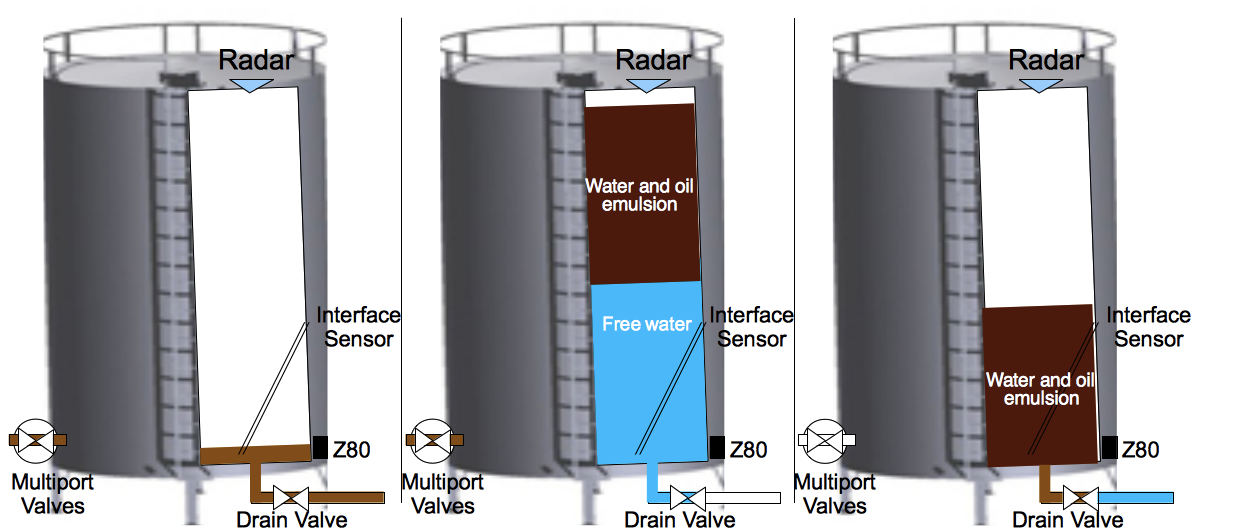
\includegraphics[width=1.\textwidth]{images/FasesEstudoDeCaso.png}
\caption{Stages of the production test.}
\label{fig:CaseStudy}
\end{figure}

% Na fase de drenagem, o nível de óleo desce relativamente rápido até aproximar-se do sensor de interface.
% Nesse instante a válvula de drenagem começa a fechar lentamente e, consequentemente, diminui a
% velocidade de  saída do fluido. Todo esse cuidado é importante para evitar a formação de vórtice\footnote{Vórtice
% é disposição concêntrica e raiada do fluido, ou seja, redemoinho ou pequenas
% ondas.}, o que afeta diretamente as propriedades do óleo extraído.


% [Dúvidas]
% - O sistema de automação usa clp (microcontrolador), ok? Sim Onde? No controle da válvulas, no recebimento das
% informações e cálculo de nível. Mais detalhes podem ser obtidos na dissertacao de LIMA
% - O  computador supervisório ? Apenas monitora e envia comandos! O microcontrolador é quem trabalha mesmo! Mais
% metalhes na {LAUT_LIMA}
% - 

%\begin{figure}[h]
%\centering 
%\includegraphics[width=.8\textwidth]{images/fluxograma_teste_drenagem.png}
%\includegraphics[width=0.95\textwidth]{images/diagrama_de_atividades.png}
%\caption{Diagrama de atividades do sistema de controle da válvula de drenagem do teste de produção
%\cite{LAUT_SERGIO}.}

%\label{fig:FluxogramaEstudoDeCaso}
%\end{figure}

%A Figura~\ref{fig:FluxogramaEstudoDeCaso} mostra o diagrama de atividades sobre o sistema de controle da
%válvula de drenagem.
% Contudo, para melhor entender o diagrama é necessário conhecer alguns conceitos: BSW
%é a abreviação de \textit{Basic Sediments and Water} e mede a proporção de água e sedimentos no fluído
%extraído; BSWe mede a proporção do volume de água contido na emulsão água e óleo entre o volume total
%dessa emulsão; CW (\textit{cut water}) representa a capacidade do óleo emulsionado reter mais ou menos
%água. De acordo com \cite{LAUT_SERGIO}, o CW é definido no programa como 20\% ou 40\%, conforme a
%densidade do fluido; e esses valores foram pré-definidos após experimentos em campo. O sistema de controle
%da válvula de drenagem começa inicializando as variáveis do sistema, esses valores são ajustados de acordo
%com o teste realizado anteriormente e experimentos. Em seguida, o sistema passa a monitorar o estado do
%sensor e do radar. O sistema vai ajustando lentamente o nível de abertura da válvula de drenagem até o
%sensor de interface identificar óleo. Finalmente, o processo de teste termina.

% Paragrafo de acima adaptado em baixo

%Para melhor entender a fase de drenagem é importante conhecer o conceito de
%BSW, a abreviação de
%\textit{Basic Sediments and Water}, que representa a proporção de água e
%sedimentos no fluído extraído.
%; BSWe
%mede a proporção do volume de água contido na emulsão água e óleo entre o volume total dessa emulsão;
% CW (\textit{cut water}) representa a capacidade do óleo emulsionado reter mais ou menos água. De acordo
% com \cite{LAUT_SERGIO}, o CW é definido no programa como 20\% ou 40\%, conforme a densidade do fluido; e
% esses valores foram pré-definidos após experimentos em campo.
%De acordo com o valor do BSW histórico do poço e outras propriedades do
%fluído, o sistema estima o nível da interface água e óleo.
% O sistema de controle da válvula de drenagem começa inicializando as variáveis do sistema, esses valores
% são ajustados de acordo com o teste realizado anteriormente e experimentos.
%Em seguida, o sistema passa a controlar a válvula de drenagem e a monitorar o
%estado do sensor e do radar. O sistema vai ajustando lentamente o nível de
%abertura da válvula de drenagem até o sensor de interface identificar a emulsão
%água e óleo. Finalmente, o processo de teste termina.

% % Motivação para o que pretendemos modelar
% Como uma medição exata reduz sensivelmente a margem de erro,
% a técnica desenvolvida por \cite{LAUT_SERGIO} pretende identificar com boa
% exatidão o atual nível da lámina de óleo através das informações seguintes:
% valor do sensor de interface,  ní­vel do tanque obtido pelo radar e outros
% parâmetros obtidos através de experimentos. Porém, uma garantia matemática sobre
% o correto funcionamento do sistema é fundamental. Assim, um cuidado especial deve ser
% realizado nesse sistema.

% % De que forma ?  O sistema verificado pode atuar ? Como um sistema redundante, visto o grau de confiança
% Para essa finalidade, um \textit{software} foi especificado, verificado, implementado e simulado. A princípio, o \textit{software}
% desenvolvido pode atuar como um sistema redundante na plataforma Z80 para interagir com os dispositivos e o sistema supervisório.
% Esse \textit{software} apenas realiza um cálculo relativo a produção de óleo, com a finalidade de avaliar se o sistema está funcionando corretamente.


B models were created to represent partially the production test system. This
report shows, in \ref{sec:Bmodel_case_study},  the main part of specification
system is organized in three different B models: \textit{TestCalc},
\textit{TestCalc\_i} and \textit{TestCalc\_basm}.

%  This specification is small and simplified, because its main objective
% is to demonstrate the technique of verification up to assembly level.

% O que pretende-se modelar ? O que foi feito ?
%Assim, o software foi implementado em \textit{assembly} e simulado um
%\textit{software} para calcular um fator de proporção de óleo bruto e água livre.

% Aparentemente, o projeto de desenvolvimento desse \textit{software} é uma atividade relativamente simples,
% porém como a técnica de verificação utilizada até o nível de \textit{assembly} é completamente inovadora,
% então surgiram algumas dificuldades iniciais que levaram tempo para ser solucionadas. A seção seguinte
% apresenta mais detalhes sobre a modelagem desse \textit{software}. 
% Essas funcionalidades foram modeladas em B
% e apresentadas nas duas seções seguintes.




%[explicar as conexão/comunicação entre os dispositivos]
 % Para realizar a comunicação entre os dispositivos serão utilizados conversores analógico/digital. 
 % As informações estão representanda em 8 bits.
 % Explicar o Wait bit de espera :D

% \subsection{Modelagem B do controle da válvula de drenagem}
% \label{sec:Modelagem B do controle da válvula de drenagem}
% 
% %[Explicar o objetivo do modelo]- princ
% [Rascunho]
% O obejtivo principal da modelagem apresentada nesta seção é especificar a parte essencial do controle da
% válvula de drenagem. Como visto anteriormente na fase de drenagem, essa válula  varia o
% estado de abertura de acordo com dois critérios: o nível da lámina de óleo ou sensor de interface, o qual 
% identifica óleo ou água no fundo do tanque. Considerando que se o sensor de interface
% indica a presença de óleo, então o sistema deve fechar a válvula do dreno. Caso contrário, ou seja,
% indica a presença de água livre, então o sistema deve ajustar a abertura da válvula proporcionalmente ao
% nível de água livre.
% 
% 
% % O software que faz controle da válvula de drenagem pode ser separado em três partes:
% % Cálculo do nível inicial ( multiplicação e condicional \ldots )
% % Atualização do nível inicial ( Uma subtração e atualização da variável )
% % Controle da abertura da válvula ( Atualização do controle da válvula )
% % A modelagem dessa seção preocupa-se com o controle da válvula de abertura.
% 
% 
% Como visto na Figura \ref{fig:FluxogramaEstudoDeCaso} o valor da válvula é atualizado aproximadamente em
% intervalos de 15 cm. Contudo, segundo \cite{LAUT_SERGIO}  é sugerido o uso de uma função do tipo rampa
% $valve=k*t$, a fim de evitar fechamentos bruscos. Onde, $valve$ é o percentual de abertura, $k$ é uma
% constante e $t$ é o tempo. Baseado na função utilizada atualmente, sugiro a seguinte função: $valve = k*H
% + c1$. Onde, $H$ é o nível de água livre, $k$ é igual à  $0,5$ e $c1$ é uma constante para abertura
% adicional, o qual pode ser ajustado para evitar um tempo excessivo no processo de drenagem. 
% 
% A Figura~\ref{fig:GraficoFuncoes} ilustra as funções de controle da válvula de drenagem, o eixo vertical
% representa o percentual de abertura da válvula de drenagem e o eixo horizontal representa $H$ (o nível de
% água livre), o que é inversamente proporcional ao tempo de drenagem.
% 
% A função representada em linha azul é a utilizada atualmente, a mesma descrita na Figura 
% \ref{fig:FluxogramaEstudoDeCaso}. A representada em linha vermelha é a proposta por esse trabalho, essa
% possui uma maior abertura inicial (100\%) e fechamento mais suave, o que reduz o tempo de
% drenagem e evita a formação de vórtice.
% 
% 
% \begin{figure}[h]
% \centering 
% %\includegraphics[width=.8\textwidth]{images/fluxograma_teste_drenagem.png}
% \includegraphics[width=0.99\textwidth]{images/Grafico_funcoes_da_valvula.png}
% \caption{Gráfico das funções que controla a válvula de drenagem..}
% 
% \label{fig:GraficoFuncoes}
% \end{figure}
% 
% Manipulando a função ($valve = 0.5*H + c1$) e substituindo $H$ pelo parámetro $level$ temos a seguinte
% função $valve = level/2 + c1$. O sistema também deve levar em consideração a informação obtida pelo
% sensor de interface, o que informa a presença de água livre no fundo do tanque. Dessa forma, a operação
% B seguinte modela essa funcionalidade. A operação ``ControlValve'' recebe como parámetro o nível de água
% livre ($level$) e o parámetro ($water$) para calcular a abertura da válvula de drenagem adequada.
% 
% \begin{tabular}[c]{l}
% \hspace*{0.20in}\bf ControlValve\rm (\it level\rm , \it water\rm )\rm =\\
% \hspace*{0.20in}\bf PRE\\
% \hspace*{0.40in}\it level\hspace*{0.10in} $\in$  \rm 0 $\upto$ \rm 2\rm 0\rm 0  $\land$  \it water 
% $\in$  \rm 0 $\upto$ \rm 1\\
% \hspace*{0.20in}\bf THEN\\
% \hspace*{0.40in}\bf IF \it water \rm = \rm 1 \bf THEN \it valve \rm := \it level $\div$ \rm 2 \rm + \it
% c1\\
% \hspace*{0.40in}\bf ELSE \it valve\rm :=\rm 0 \bf END\\
% \hspace*{0.20in}\bf END
% \end{tabular}
% 
% O primeiro refinamento dessa operação para o nível de assembly é representado a seguir no texto.
% Um fato interessante é que ele aproveita-se da propriedade da representação em \textit{bits}. Essa
% propriedade diz que a rotação à  direita de um vetor de bits é semánticamente equivalente à  divisão por
% $2^{n}$, onde $n$ é o número de rotações. Na operação de rotação $\textit{rotateright}$ $n$ é igual à  1,
% porém essa é uma rotação circular, ou seja, o bit menos significativo é copiado para o bit mais
% significativo. Para tornar a equivalente à  divisão por dois é o bit mais significativo é zerado através
% da função $\textit{bitclear}$.
% 
% \begin{tabular}[c]{l}
% \hspace*{0.15in}\bf ControlValve \rm ( \it level \rm , \it water \rm ) \rm =\\
% \hspace*{0.15in}\bf PRE\\
% \hspace*{0.35in}\it level  $\in$  \rm 0  $\upto$  \rm 2\rm 5\rm 5  $\land$  \it water  $\in$  \rm 0 
% $\upto$  \rm 1\\
% \hspace*{0.15in}\bf THEN\\
% \hspace*{0.35in}\bf IF \it water \rm = \rm 1\\
% \hspace*{0.35in}\bf THEN\\
% \hspace*{0.55in}\bf IF \it level  $\in$  \rm 2\rm 0\rm 1 $\upto$ \rm 2\rm 5\rm 5 \bf THEN \it valve\rm
% :=\rm 1\rm 0\rm 0\\
% \hspace*{0.55in}\bf ELSE \it valve \rm := \it byte\_uchar\rm (\it bitclear\rm (\it rotateright\rm (\it
% uchar\_byte\rm (\it level\rm )\rm )\rm ,\rm 7\rm )\rm )\rm +\it c1 \\
% \hspace*{0.55in}\bf END\\
%  \hspace*{0.35in}\bf ELSE\\
% \hspace*{0.55in}\it valve \rm := \rm 0\\
% \hspace*{0.35in}\bf END\\
% \hspace*{0.15in}\bf END\\
% \end{tabular}
% 
% 
% A seguir é ilustrado o modelo em nível de assembly. 
% \begin{tabular}[c]{l}
% \ldots
% \end{tabular}
% 
% 
% Esse cógigo assembly foi simulado em \cite{Simulator_z80}. A Figura\ref{fig:control_valvula} ilustra o
% final da execução os valores de entrada \ldots e saída \ldots
% 
% \begin{figure}[h]
% \centering 
% \includegraphics[width=0.45\textwidth]{images/Simulator_main.png}
% \includegraphics[width=0.45\textwidth]{images/Simulator_Execution.png}
% \includegraphics[width=0.45\textwidth]{images/Simulator_IO_ports.png}
% \includegraphics[width=0.45\textwidth]{images/Simulator_Peripheral_Devices.png}
% \caption{Simulação do controle da válvula de drenagem.}
% \label{fig:control_valvula}
% \end{figure}
% 
% 
% 
% [abstrações]- princ 
% 
% [explicar a modelagem]
% Quais as entradas e saídas do programa ?
% [Colocar as images de simulação do Z80]
% [explicar as estátisticas] [Explicar as dificuldades] 
% [explicar as regras utilizadas]
% % DICAS PARA DISSERTAÇÃO
% % 
% % -> Explicar uma das maiores dificuldades atuais! Que é a pouca simplificação realizada, o histórico que é mantido!
% % A simplificação das expressões poderia ser mais específica. As regras de simplificação utilizadas no AtelierB muitas vezes perdem "informações importantes".
% % [Colocar um exemplo pequeno antes da simplificação e após a simplificação.]
% % 
% % Existem duas solu
% % - Simplifificar utilizando novas regras
% % - Utilizar o ambiente do ABTools e aproveitar o gerador de obrigações de prova e simplificar as expressões.
% % 
% % 
% % Vantagens em calcular somente o nível:
% % - Pode-se se adequar a qualquer tamanho de tanque.
% % Assim, o nível e o determinado tanque que deve informar a quantidade de óleo produzido.
% % 
% % Posso pegar as obrigações de prova e tentar explicar o que é provado!?!
% % * Na documentação colocar o número de provas óbvias e não obvias
% % 
% % -> Na conclusão colocar o número total de obrigações de provas não obvias realizadas!!!

\subsection{B modelling} 
%e o \textit{software} do cálculo dos fatores de óleo bruto e água livre produzidos}
\label{sec:Bmodel_case_study}

% Overview 
% [Explicar o objetivo do modelo]- princ
% [explicar a modelagem]
% - inicial, implementação, explicar o que refinamento garante,  e assembly código, explicar o
% invariante, as entradas e saidas.
% [explicar as estátisticas]
% [Processo de prova](Pouca coisa,algumas linhas) citar o comando que resolveu 465 automaticamente entre
% 568, é explicado em anexo.
% [Simulação]
% Explicar as images, a entrada e saída \ldots
% [Conclusões]
%
 

% % Overview A presente seção apresenta a modelagem B e o \textit{software} do
% cálculo do fator de proporção de óleo bruto (emulsão água e óleo) e  água livre
% produzidos.

This section shows the B modelling and the embedded software that calculates the
proportion of water and oil emulsion produced.

% % [Ressalva -> onde tiver nível substituir por proporção]
% Os fatores de proporção de óleo bruto e água livre são determinados através de informações obtidas na
% fase de drenagem. As informações utilizadas são os níveis do tanque: inicial (tanque cheio) e final (tanque com
% apenas óleo bruto) da fase de drenagem.Portanto, a subtração desse dois valores determina um fator de
% proporção de água livre produzida e o nível final do tanque determina um fator de proporção de óleo bruto
% produzido.Para determinar exatamente a quantidade de óleo e água livre, é necessário que o resultado
% seja multiplicado por um fator de correção, o qual deve representar as distorções e o formato do tanque,
% já que o tanque não tem um formato perfeitamente cilíndrico. Dessa forma, esse \textit{software}
% embarcado torna-se genérico para qualquer formato de tanque.

The proportion of factors of water and oil emulsion are estimated by collected
information in the draining stage. The information used are the levels of the
tank: initial level (full tank) and final level (tank with only water and oil
emulsion) from draining stage. So, the subtraction of two values determines a
proportional factor of free water proportion and the final level of tank
determines a proportional factor of produced water and oil emulsion (crude oil).
To determine exactly the quantity of oil emulsion and water free, it is needed to
multiply the levels by the correction factor, which represents the format of the
tank and its deformations, because the tank has not a perfectly cylindrical
shape. Thus, the final embedded software becomes generic for any tank shapes.


% Modelagem funcional
% A modelagem é iniciada com o modelo funcional \textit{TestCalc}. Esse modelo contém duas variáveis
% \textit{oil\_factor} e \textit{free\_water\_factor} que representam respectivamente o fator final de óleo e
% o de água livre. A seguir, é apresentado o invariante e a operação do modelo funcional. O invariante
% declara o tipo das variáveis como $\textit{UCHAR}$, um inteiro positivo de 8 \textit{bits}, ou seja, pertencente ao
% intervalo de 0 até 255. 
%A operação recebe como parámetro o valor inicial e final do nível do tanque e
% então calcula o fator de óleo e água livre. Uma pré-condição dessa operação é que o nível inicial do
% tanque cheio deve ser maior ou igual ao nível após a remoção da água livre. Isso é uma simplificação e 
% evita que seja realizado tratamento de exceção até o nível de \textit{assembly} para esse código.

% Functional modelling
The modelling is started in the functional model \textit{TestCalc}. This model
has two important variables \textit{oil\_factor} and \textit{free\_water\_factor}
that represent, respectively, the final oil factor and the free water factor. The
\textit{Invariant} and the operation of functional model. The \textit{Invariant}
declares the types of variables as $\textit{UCHAR}$, a positive integer value
with 8 bits, in other words, it represents the positive integers between 0 up to
255. The operation receives as a parameter the initial value and final value of
the tank, then, the software calculates the oil factor and free water factor. A
precondition of this operation is that the initial level of full tank is bigger
or equal than the level after the draining stage. This precondition is a
simplification and it avoids to create exceptions up to the assembly level.


\small{
\begin{sloppypar}
%\bf MACHINE\\
%\hspace*{0.20in}\it TestCalc\\
% \bf SEES\\
% \hspace*{0.20in}\it SCHAR\_DEFINITION\rm , \it UCHAR\_DEFINITION\\
% \bf VARIABLES\\
% \hspace*{0.20in}\it oil\_factor\rm ,\it free\_water\_factor\\
\hspace*{-0.30in}\bf INVARIANT\\
\hspace*{0.40in}\it oil\_factor  $\in$  \it UCHAR  $\land$  \it free\_water\_factor  $\in$  \it UCHAR\\
\bf OPERATIONS\\
\hspace*{0.20in}\bf update\_factor\rm (\it initial\_level\rm , \it final\_level\rm ) \rm =\\
\hspace*{0.20in}\bf PRE\\ 
\hspace*{0.40in}\it initial\_level  $\in$  \it UCHAR  $\land$  \it final\_level\hspace*{0.10in} $\in$ 
\it UCHAR  $\land$\\
\hspace*{0.40in}\it final\_level  $\leq$  \it initial\_level\\ 
\hspace*{0.20in}\bf THEN\\
\hspace*{0.40in}\it free\_water\_factor \rm := \it initial\_level \rm - \it final\_level $\para$\\ 
\hspace*{0.40in}\it oil\_factor \rm := \it final\_level\\
\hspace*{0.20in}\bf END
%\bf END\\
\end{sloppypar}
}

%A operação \textit{update\_factor} do modelo funcional \textit{TestCalc} é similar à 
%sua modelagem algorítmica, exceto o fato das substituições não acontecerem em paralelo, mas acontecem
%em sequência no modelo algorítmico, então o refinamento da modelagem algorítmica foi verificado e a sua 
%apresentação é omitida aqui.

The operation \textit{update\_factor} of functional model \textit{TestCalc} is
too much similar to its algorithmic modell, then the algorithmic modell was
developed, verified and its presentation is omitted here.


% 
% \small{
% \begin{sloppypar}
% \bf INVARIANT\\
% \hspace*{0.20in}\it oil\_factor  $\in$  \it UCHAR  $\land$  \it free\_water\_factor $\in$ \it UCHAR\\
% \bf INITIALISATION\\
% \hspace*{0.20in}\it oil\_factor \rm := \rm 0 \rm ;\hspace*{0.20in}\it free\_water\_factor\rm :=\rm 0\\
% \bf OPERATIONS\\
% \hspace*{0.15in}
% 
% \hspace*{0.20in}\bf update\_factor\rm (\it initial\_level \rm , \it final\_level\rm ) \rm =
% 
% \hspace*{0.20in}\bf ASSERT \it initial\_level  $\in$  \it UCHAR  $\land$  \it final\_level  $\in$  \it UCHAR
% 
% \hspace*{0.45in} $\land$  \it initial\_level $\geq$  \it final\_level
% 
% \hspace*{0.20in}\bf THEN
% 
% \hspace*{0.40in}\bf BEGIN
% 
% \hspace*{0.60in}\it free\_water\_factor \rm := \it initial\_level \rm - \it final\_level\rm ;
% 
% \hspace*{0.60in}\it oil\_factor \rm := \it final\_level
% 
% \hspace*{0.40in}\bf END
% 
% \hspace*{0.20in}\bf END
% \end{sloppypar}
% }

%Parte da modelagem B no nível de \textit{assembly} é representada a seguir. Ela é especificada no modelo
%\textit{TestCalc\_basm} e possui a mesma semántica de manipulação das variáveis que o modelo abstrato
%(\textit{TestCalc}), entretanto utiliza operações que representam instruções \textit{assembly} de
%uma instáncia do modelo do Z80 para manipular a sua memória. 

Part of B modelling in assembly level is shown as it follows. It is specified in
the model \textit{TestCalc\_basm} and it has the same semantic of manipulation of
variables that the abstract model (\textit{TestCalc}), however it uses operations
that represent the assembly instructions of an instance of Z80 model to
manipulate its memory.


%A cláusula invariante estabelece a relação das variáveis do modelo inicial (\textit{free\_water\_factor} e
%\textit{oil\_factor}) com os valores dos endereços 2 e 3 da porta de entrada e saída; para estabelecer
%essa relação são utilizadas funções que convertem valores da representação binária para representação de
%inteiro e vice-versa. Dessa forma, a verificação do refinamento garante que as operações do modelo B
%\textit{assembly} são semánticamente equivalentes  Ã s operações do modelo mais abstrato de acordo com a
%relação estabelecida entre as variáveis no invariante.

The \textit{Invariant} clause  determines the relation of variables of initial model (\textit{free\_water\_factor}
and \textit{oil\_factor}) to the values from address 2 and 3 from I/O port; to determine the relation are used functions
that convert values between binary representation and integer representation.

\small{
\begin{sloppypar}
\hspace*{-0.30in}\bf IMPORTS\\
\hspace*{0.20in}\it Z80\\
\bf INVARIANT\\
\hspace*{0.20in}\it byte\_uchar\rm (\it io\_ports\rm (\it uchar\_byte\rm (\rm 2\rm )\rm )\rm ) \rm
=\hspace*{0.10in}\rm (\it free\_water\_factor \rm )  $\land$\\
\hspace*{0.20in}\it byte\_uchar\rm (\it io\_ports\rm (\it uchar\_byte\rm (\rm 3\rm )\rm )\rm ) \rm
=\hspace*{0.10in}\rm (\it oil\_factor\rm )
% \bf INITIALISATION\\
% \hspace*{0.20in}\it ext\_update\_io\_ports\rm (\rm 2\rm ,\it uchar\_schar\rm (\rm 0\rm )\rm )\rm ;\\
% \hspace*{0.20in}\it ext\_update\_io\_ports\rm (\rm 3\rm ,\it uchar\_schar\rm (\rm 0\rm )\rm )\\
\end{sloppypar}
}

% % entrada e saida%
% A seguir é apresentada a operação $\textit{update\_factor}$ utilizando instruções em nível de
% \textit{assembly}. Essa operação possui a mesma assinatura que o modelo mais abstrato, e os parámetros
% recebidos são convertidos para representação em binário e passados para a operação de atualização das
% portas do microcontrolador ($\textit{ext\_update\_io\_ports}$).
% %Explicação geral do program
% Sucintamente, a sequência de instruções ilustradas a seguir realiza os seguintes procedimentos. As cinco
% primeiras instruções representam apenas a cópia dos dados externos ao microcontrolador para os
% registradores de memória ``A'' e ``C''. A instrução seguinte realiza uma subtração, então as demais copiam
% os fatores de proporção de água livre e óleo bruto respectivamente para as portas 2 e 3. O leitor pode
% consultar o anexo desse trabalho para entender detalhes da especificação de cada instrução e o invariante
% completo da operação $\textit{update\_factor}$ ilustrada a seguir.

Below is presented the operation $\textit{update\_factor}$ using the instructions
in the assembly level. This operation has the same signature as the most
abstract model and the parameters received are converted to binary representation and
transfered to the updated operation of the ports of the microcontroller
($\textit{ext\_update\_io\_ports}$).

Briefly, the sequence of instructions illustrated performs the following
procedures. The first three instructions are representing just copying the data
from external input and output ports to memory registers ``A'' and ``C''. The
following instruction performs a subtraction, then copies the other factors
proportion of free water and crude oil, respectively, to ports 2 and 3. The
reader may consult the site repository of this work to know more details about the
specification of each statement and the complete $\textit{update\_factor}$
operation.
   
% Explicação sobre a construção do invariant
\newpage \small{
\begin{sloppypar}
%\hspace*{0.20in}\bf OPERATIONS\\
\hspace*{-0.30in}\bf update\_factor\rm (\it initial\_level\rm , \it final\_level\rm ) \rm =\\
\hspace*{0.20in}\it ASSERT\\ 
\hspace*{0.40in}\it initial\_level  $\in$  \it UCHAR  $\land$  \it final\_level\hspace*{0.10in} $\in$ 
\it UCHAR%\\
\hspace*{0.00in} $\land$  \it final\_level  $\leq$  \it initial\_level\\ 
\hspace*{0.20in}\bf THEN\\
\hspace*{0.40in}\bf VAR \it local\_pc \bf IN
\hspace*{0.20in}\it local\_pc \rm := \rm 0\rm ;
\hspace*{0.20in}\bf set\_pc\rm (\it local\_pc\rm )\rm ;\\
\hspace*{0.60in}\bf WHILE \it local\_pc $<$ \rm 9 \bf DO\\
\hspace*{0.80in}\bf CASE \it local\_pc \bf OF\\
\hspace*{1.00in}\bf EITHER \rm 0 \bf THEN
\bf ext\_update\_io\_ports\rm (\rm 0\rm ,\it uchar\_schar\rm (\it initial\_level\rm )\rm
)\rm ;\\
\hspace*{2.45in}\bf IN\_A\_9n0\rm (\rm 0\rm )\\
\hspace*{1.00in}\bf OR \rm 1 \bf THEN\hspace*{0.50in}\bf LD\_r\_r\_\rm (\it b0\rm ,\it a0\rm )\\
\hspace*{1.00in}\bf OR \rm 2 \bf THEN
\hspace*{0.47in}\bf ext\_update\_io\_ports\rm (\rm 1\rm ,\it uchar\_schar\rm (\it final\_level\rm
)\rm)\rm ;\\ \hspace*{2.47in}\bf IN\_A\_9n0\rm (\rm 1\rm )\\
\hspace*{1.00in}\bf OR \rm 3 \bf THEN \hspace*{0.47in}\bf LD\_r\_r\_\rm (\it c0\rm ,\it a0\rm )\\
\hspace*{1.00in}\bf OR \rm 4 \bf THEN \hspace*{0.47in}\bf LD\_r\_r\_\rm (\it a0\rm ,\it b0\rm )\\
\hspace*{1.00in}\bf OR \rm 5 \bf THEN \hspace*{0.47in}\bf SUB\_A\_r\rm (\it c0\rm )\\
\hspace*{1.00in}\bf OR \rm 6 \bf THEN \hspace*{0.47in}\bf OUT\_9n0\_A\rm (\rm 2\rm )\\ 
\hspace*{1.00in}\bf OR \rm 7 \bf THEN \hspace*{0.47in}\bf LD\_r\_r\_\rm (\it a0\rm ,\it c0\rm )\\
\hspace*{1.00in}\bf OR \rm 8 \bf THEN \hspace*{0.47in}\bf OUT\_9n0\_A\rm (\rm 3\rm )\\ 
\hspace*{1.00in}\bf END
\hspace*{0.20in}\bf END\rm ;
\hspace*{0.20in}\it local\_pc  $\leftarrow$  \bf get\_pc\\
\hspace*{0.70in}\bf INVARIANT\\
\hspace*{0.80in}\it local\_pc  $\in$  \rm 0 $\upto$ \rm 9  $\land$  \it rgs8  $\in$  \it id\_reg\_8 
$\fun$  \it BYTE\\
\hspace*{0.80in} $\land$  \it r\_\hspace*{0.10in} $\in$  \it BYTE  $\land$  \it io\_ports  $\in$  \it
BYTE  $\fun$  \it BYTE\\
\hspace*{0.80in} $\land$  \it pc  $\in$  \rm 0 $\upto$ \rm 9  $\land$  \it free\_water\_factor  $\in$ 
\it UCHAR  $\land$\\
\hspace*{0.80in}\rm (\it local\_pc \rm = \rm 0  $\implies$  \rm ( \it pc \rm = \rm 0  $\land$  \it
instruction\_next\rm (\it pc\rm ) \rm = \rm 1  $\land$\\
\hspace*{1.10in}\it byte\_uchar\rm (\it io\_ports\rm (\it uchar\_byte\rm (\rm 2\rm )\rm )\rm ) \rm
=\hspace*{0.10in}\it free\_water\_factor  $\land$\\
\hspace*{1.10in}\it byte\_uchar\rm (\it io\_ports\rm (\it uchar\_byte\rm (\rm 3\rm )\rm )\rm ) \rm
=\hspace*{0.10in}\it oil\_factor \rm ) $\land$\\
\hspace*{1.10in}\ldots\\ 
% \hspace*{0.80in}\rm (\it local\_pc \rm = \rm 1  $\implies$  \rm ( \it instruction\_next\rm (\it pc\rm )
% \rm = \rm 2  $\land$\\
% \hspace*{1.10in}\it byte\_uchar\rm (\it io\_ports\rm (\it uchar\_byte\rm (\rm 0\rm )\rm )\rm ) \rm
% =\hspace*{0.10in}\it initial\_level  $\land$\\
% \hspace*{1.10in}\it byte\_uchar\rm ( \it rgs8\rm (\it a0\rm ) \rm ) \rm = \rm ( \it initial\_level \rm
% )\hspace*{0.15in} $\land$\\
% \hspace*{1.10in}\it byte\_uchar\rm (\it io\_ports\rm (\it uchar\_byte\rm (\rm 2\rm )\rm )\rm ) \rm
% =\hspace*{0.10in}\it free\_water\_factor  $\land$\\
% \hspace*{1.10in}\it byte\_uchar\rm (\it io\_ports\rm (\it uchar\_byte\rm (\rm 3\rm )\rm )\rm ) \rm
% =\hspace*{0.10in}\it oil\_factor \rm ) \rm ) $\land$\\
% \hspace*{0.80in}\rm (\it local\_pc \rm = \rm 2  $\implies$  \rm ( \it instruction\_next\rm (\it pc\rm )
% \rm = \rm 3  $\land$\\
% \hspace*{1.10in}\it byte\_uchar\rm (\it io\_ports\rm (\it uchar\_byte\rm (\rm 0\rm )\rm )\rm ) \rm
% =\hspace*{0.10in}\it initial\_level  $\land$\\
% \hspace*{1.10in}\it byte\_uchar\rm ( \it rgs8\rm (\it b0\rm ) \rm ) \rm = \rm ( \it initial\_level \rm )
% $\land$\\
% \hspace*{1.10in}\it byte\_uchar\rm ( \it rgs8\rm (\it a0\rm ) \rm ) \rm = \rm ( \it initial\_level \rm )
% $\land$\\
% \hspace*{1.10in}\it byte\_uchar\rm (\it io\_ports\rm (\it uchar\_byte\rm (\rm 2\rm )\rm )\rm ) \rm
% =\hspace*{0.10in}\it free\_water\_factor  $\land$\\
% \hspace*{1.10in}\it byte\_uchar\rm (\it io\_ports\rm (\it uchar\_byte\rm (\rm 3\rm )\rm )\rm ) \rm
% =\hspace*{0.10in}\it oil\_factor \rm ) \rm ) $\land$\\
% \hspace*{0.80in}\rm (\it local\_pc \rm = \rm 3  $\implies$  \rm ( \it instruction\_next\rm (\it pc\rm )
% \rm = \rm 4  $\land$\\
% \hspace*{1.10in}\it byte\_uchar\rm (\it io\_ports\rm (\it uchar\_byte\rm (\rm 0\rm )\rm )\rm ) \rm
% =\hspace*{0.10in}\it initial\_level  $\land$\\
% \hspace*{1.10in}\it byte\_uchar\rm (\it io\_ports\rm (\it uchar\_byte\rm (\rm 1\rm )\rm )\rm ) \rm
% =\hspace*{0.10in}\it final\_level  $\land$ \\
% \hspace*{1.10in}\it byte\_uchar\rm ( \it rgs8\rm (\it a0\rm ) \rm ) \rm = \rm ( \it final\_level \rm ) 
% $\land$\\
% \hspace*{1.10in}\it byte\_uchar\rm ( \it rgs8\rm (\it b0\rm ) \rm ) \rm = \rm ( \it initial\_level \rm )
% $\land$\\
% \hspace*{1.10in}\it byte\_uchar\rm (\it io\_ports\rm (\it uchar\_byte\rm (\rm 2\rm )\rm )\rm ) \rm
% =\hspace*{0.10in}\it free\_water\_factor  $\land$\\
% \hspace*{1.10in}\it byte\_uchar\rm (\it io\_ports\rm (\it uchar\_byte\rm (\rm 3\rm )\rm )\rm ) \rm
% =\hspace*{0.10in}\it oil\_factor \rm ) \rm ) $\land$\\
% \hspace*{0.80in}\rm (\it local\_pc \rm = \rm 4  $\implies$  \rm ( \it instruction\_next\rm (\it pc\rm )
% \rm = \rm 5  $\land$\\
% \hspace*{1.10in}\it byte\_uchar\rm (\it io\_ports\rm (\it uchar\_byte\rm (\rm 0\rm )\rm )\rm ) \rm
% =\hspace*{0.10in}\it initial\_level  $\land$\\
% \hspace*{1.10in}\it byte\_uchar\rm (\it io\_ports\rm (\it uchar\_byte\rm (\rm 1\rm )\rm )\rm ) \rm
% =\hspace*{0.10in}\it final\_level  $\land$ \\
% \hspace*{1.10in}\it byte\_uchar\rm ( \it rgs8\rm (\it a0\rm ) \rm ) \rm = \rm ( \it final\_level \rm ) 
% $\land$\\
% \hspace*{1.10in}\it byte\_uchar\rm ( \it rgs8\rm (\it c0\rm ) \rm ) \rm = \rm ( \it final\_level \rm ) 
% $\land$\\
% \hspace*{1.10in}\it byte\_uchar\rm ( \it rgs8\rm (\it b0\rm ) \rm ) \rm = \rm ( \it initial\_level \rm )
% $\land$\\
% \hspace*{1.10in}\it byte\_uchar\rm (\it io\_ports\rm (\it uchar\_byte\rm (\rm 2\rm )\rm )\rm ) \rm
% =\hspace*{0.10in}\it free\_water\_factor  $\land$\\
% \hspace*{1.10in}\it byte\_uchar\rm (\it io\_ports\rm (\it uchar\_byte\rm (\rm 3\rm )\rm )\rm ) \rm
% =\hspace*{0.10in}\it oil\_factor \rm ) \rm ) $\land$\\
% \hspace*{0.80in}\rm (\it local\_pc \rm = \rm 5\hspace*{0.10in} $\implies$  \rm ( \it
% instruction\_next\rm (\it pc\rm ) \rm = \rm 6  $\land$\\
% \hspace*{1.10in}\it byte\_uchar\rm (\it io\_ports\rm (\it uchar\_byte\rm (\rm 0\rm )\rm )\rm ) \rm
% =\hspace*{0.10in}\it initial\_level  $\land$\\
% \hspace*{1.10in}\it byte\_uchar\rm (\it io\_ports\rm (\it uchar\_byte\rm (\rm 1\rm )\rm )\rm ) \rm
% =\hspace*{0.10in}\it final\_level  $\land$ \\
% \hspace*{1.10in}\it byte\_uchar\rm ( \it rgs8\rm (\it a0\rm ) \rm ) \rm = \rm ( \it initial\_level \rm )
% $\land$\\
% \hspace*{1.10in}\it byte\_uchar\rm ( \it rgs8\rm (\it c0\rm ) \rm ) \rm = \rm ( \it final\_level \rm ) 
% $\land$\\
% \hspace*{1.10in}\it byte\_uchar\rm ( \it rgs8\rm (\it b0\rm ) \rm ) \rm = \rm ( \it initial\_level \rm )
% $\land$\\
% \hspace*{1.10in}\it byte\_uchar\rm (\it io\_ports\rm (\it uchar\_byte\rm (\rm 2\rm )\rm )\rm ) \rm
% =\hspace*{0.10in}\it free\_water\_factor  $\land$\\
% \hspace*{1.10in}\it byte\_uchar\rm (\it io\_ports\rm (\it uchar\_byte\rm (\rm 3\rm )\rm )\rm ) \rm
% =\hspace*{0.10in}\it oil\_factor \rm ) \rm ) $\land$ \\
% \hspace*{0.80in}\rm (\it local\_pc \rm = \rm 6\hspace*{0.10in} $\implies$  \rm ( \it
% instruction\_next\rm (\it pc\rm ) \rm = \rm 7  $\land$\\
% \hspace*{1.10in}\it byte\_uchar\rm (\it io\_ports\rm (\it uchar\_byte\rm (\rm 0\rm )\rm )\rm ) \rm
% =\hspace*{0.10in}\it initial\_level  $\land$ \\
% \hspace*{1.10in}\it byte\_uchar\rm (\it io\_ports\rm (\it uchar\_byte\rm (\rm 1\rm )\rm )\rm ) \rm
% =\hspace*{0.10in}\it final\_level  $\land$ \\
% \hspace*{1.10in}\it byte\_uchar\rm ( \it rgs8\rm (\it a0\rm ) \rm ) \rm = \rm ( \rm (\it initial\_level
% \rm - \it final\_level\rm )  $\mod$  \rm 2\rm 5\rm 6\rm )  $\land$\\
% \hspace*{1.10in}\it byte\_uchar\rm ( \it rgs8\rm (\it c0\rm ) \rm ) \rm = \rm ( \it final\_level \rm ) 
% $\land$\\
% \hspace*{1.10in}\it byte\_uchar\rm ( \it rgs8\rm (\it b0\rm ) \rm ) \rm = \rm ( \it initial\_level \rm )
% $\land$\\
% \hspace*{1.10in}\it byte\_uchar\rm (\it io\_ports\rm (\it uchar\_byte\rm (\rm 2\rm )\rm )\rm ) \rm
% =\hspace*{0.10in}\it free\_water\_factor  $\land$\\
% \hspace*{1.10in}\it byte\_uchar\rm (\it io\_ports\rm (\it uchar\_byte\rm (\rm 3\rm )\rm )\rm ) \rm
% =\hspace*{0.10in}\it oil\_factor \rm ) \rm ) $\land$\\
% \hspace*{0.80in}\rm (\it local\_pc \rm = \rm 7\hspace*{0.10in} $\implies$  \rm ( \it
% instruction\_next\rm (\it pc\rm ) \rm = \rm 8  $\land$\\
% \hspace*{1.10in}\it byte\_uchar\rm (\it io\_ports\rm (\it uchar\_byte\rm (\rm 0\rm )\rm )\rm ) \rm
% =\hspace*{0.10in}\it initial\_level  $\land$ \\
% \hspace*{1.10in}\it byte\_uchar\rm (\it io\_ports\rm (\it uchar\_byte\rm (\rm 1\rm )\rm )\rm ) \rm
% =\hspace*{0.10in}\it final\_level  $\land$\\
% \hspace*{1.10in}\it byte\_uchar\rm ( \it rgs8\rm (\it a0\rm ) \rm ) \rm = \rm ( \rm (\it initial\_level
% \rm - \it final\_level\rm )  $\mod$  \rm 2\rm 5\rm 6\rm )  $\land$\\
% \hspace*{1.10in}\it byte\_uchar\rm ( \it rgs8\rm (\it c0\rm ) \rm ) \rm = \rm ( \it final\_level \rm ) 
% $\land$\\
% \hspace*{1.10in}\it byte\_uchar\rm ( \it rgs8\rm (\it b0\rm ) \rm ) \rm = \rm ( \it initial\_level \rm )
% $\land$\\
% \hspace*{1.10in}\it byte\_uchar\rm (\it io\_ports\rm (\it uchar\_byte\rm (\rm 2\rm )\rm )\rm ) \rm
% =\hspace*{0.10in}\rm (\rm (\it initial\_level \rm - \it final\_level\rm )  $\mod$  \rm 2\rm 5\rm 6\rm )
% $\land$\\
% \hspace*{1.10in}\it byte\_uchar\rm (\it io\_ports\rm (\it uchar\_byte\rm (\rm 3\rm )\rm )\rm ) \rm
% =\hspace*{0.10in}\it oil\_factor  $\land$\\
% \hspace*{0.80in}\rm (\it local\_pc \rm = \rm 8\hspace*{0.10in} $\implies$  \rm ( \it
% instruction\_next\rm (\it pc\rm ) \rm = \rm 9  $\land$\\
% \hspace*{1.10in}\it byte\_uchar\rm (\it io\_ports\rm (\it uchar\_byte\rm (\rm 0\rm )\rm )\rm ) \rm
% =\hspace*{0.10in}\it initial\_level  $\land$ \hspace*{0.20in}\\
% \hspace*{1.10in}\it byte\_uchar\rm (\it io\_ports\rm (\it uchar\_byte\rm (\rm 1\rm )\rm )\rm ) \rm
% =\hspace*{0.10in}\it final\_level  $\land$\\
% \hspace*{1.10in}\it byte\_uchar\rm ( \it rgs8\rm (\it a0\rm ) \rm ) \rm = \rm ( \it final\_level\rm ) 
% $\land$ \\
% \hspace*{1.10in}\it byte\_uchar\rm ( \it rgs8\rm (\it c0\rm ) \rm ) \rm = \rm ( \it final\_level \rm ) 
% $\land$\\
% \hspace*{1.10in}\it byte\_uchar\rm ( \it rgs8\rm (\it b0\rm ) \rm ) \rm = \rm ( \it initial\_level \rm )
% $\land$\\\
% \hspace*{1.10in}\it byte\_uchar\rm (\it io\_ports\rm (\it uchar\_byte\rm (\rm 2\rm )\rm )\rm ) \rm
% =\hspace*{0.10in}\rm (\rm (\it initial\_level \rm - \it final\_level\rm )  $\mod$  \rm 2\rm 5\rm 6\rm )
% $\land$\\
% \hspace*{1.10in}\it byte\_uchar\rm (\it io\_ports\rm (\it uchar\_byte\rm (\rm 3\rm )\rm )\rm ) \rm
% =\hspace*{0.10in}\it oil\_factor )  $\land$\\ 
\hspace*{0.80in}\rm (\it local\_pc \rm = \rm 9\hspace*{0.10in} $\implies$  \rm ( \it pc \rm = \rm 9 
$\land$\\
\hspace*{1.10in}\it byte\_uchar\rm (\it io\_ports\rm (\it uchar\_byte\rm (\rm 0\rm )\rm )\rm ) \rm
=\hspace*{0.10in}\it initial\_level  $\land$ \hspace*{0.20in}\\
\hspace*{1.10in}\it byte\_uchar\rm (\it io\_ports\rm (\it uchar\_byte\rm (\rm 1\rm )\rm )\rm ) \rm
=\hspace*{0.10in}\it final\_level  $\land$\\
\hspace*{1.10in}\it byte\_uchar\rm ( \it rgs8\rm (\it a0\rm ) \rm ) \rm = \rm ( \it final\_level\rm ) 
$\land$\\
\hspace*{1.10in}\it byte\_uchar\rm ( \it rgs8\rm (\it c0\rm ) \rm ) \rm = \rm ( \it final\_level \rm ) 
$\land$\\
\hspace*{1.10in}\it byte\_uchar\rm ( \it rgs8\rm (\it b0\rm ) \rm ) \rm = \rm ( \it initial\_level \rm )
$\land$\\
\hspace*{1.10in}\it byte\_uchar\rm (\it io\_ports\rm (\it uchar\_byte\rm (\rm
2\rm )\rm )\rm ) \rm =\hspace*{0.10in}\rm (\rm (\it initial\_level \rm - \it
final\_level\rm )  $\mod$  \rm 2\rm 5\rm 6\rm )\\ \hspace*{1.10in} $\land$\\
\hspace*{1.10in}\it byte\_uchar\rm (\it io\_ports\rm (\it uchar\_byte\rm (\rm 3\rm )\rm )\rm ) \rm
=\hspace*{0.10in}\it final\_level \rm )\rm )\\
\hspace*{0.70in}\bf VARIANT \rm (\rm 9 \rm - \it local\_pc\rm ) \bf END\hspace*{0.50in}\\
\hspace*{0.70in}\bf END
\hspace*{0.20in}\bf END\\
\hspace*{0.40in}\bf END
\end{sloppypar}
}


% 
% O invariante do $\WHILE$ deve formalizar o estado e o mapeamento das variáveis do modelo abstrato
% com os valores dos endereços de memória relacionado. Portanto, para cada iteração do \textit{while}, que
% é associada com o valor do contador de programa (\textit{pc}), deve existir uma expressão para realizar
% essa formalização. A cláusula variante deve expressar o limite superior do número de instruções a ser
% executado para cada valor possível do contador de programa.

The invariant from $\WHILE$ must formalize every state of execution and mapping
between the variables from the abstract model and values from memory address
related. So, for each interaction of $\WHILE$, which  is associated with a
value from the program counter (\textit{pc}). The $\VARIANT$ clause must express
the superior number of instructions to be executed for every possible value of
the program counter.


% Um detalhe interessante desse modelo é que as instruções do Z80 podem receber valores inteiros,
% porém o modelo do Z80 representa internamente os dados na notação binária. Essa diferença na representação poderia
% dificultar bastante o processo de verificação. No entanto, os tipos, as funções e os lemas construídos
% para suportar e converter as duas representações facilitaram bastante o processo de verificação.

An interesting detail of this model is  that instructions of Z80 receive integer
values, but the model of Z80 represents the data in binary notation. This
difference could become the verification process more difficult. However, the
types, functions and lemmas developed to support and to convert the data types
facilitate the verification process.

Before starting the verification process, we recommend a review of the assembly code. 
So, this can be done using the assembly code simulation.
%So, the assembly code simulation, presented in the next subsection, allows also
%to analyse and review the code implementation.


\subsection{Assembly code simulation}

%\subsection{Simulação do código assembly}

% A simulação do \textit{software}\footnote{A sequência de instruções representadas no modelo
% \textit{TestCalc\_basm} formam um \textit{software} em linguagem \textit{assembly} do Z80, o qual é
% ilustrado no lado superior direito da Figura~\ref{fig:simulacao}.} tem um papel importante para analisar
% seu comportamento, pois, no simulador, é possível avaliar e manipular os valores dos registradores, da
% memória e das portas de entrada e saída. O uso do simulador permite ganhar confiança no programa \textit{assembly}
% desenvolvido, assim como no próprio modelo formal do conjunto de instruções do Z80, visto que o manual
% possui pequenos erros.
The assembly code simulation is important to analyse its behavior, because the
simulator allows to evaluate and to manipulate the state data (memory, registers and I/O ports) and execution flow.
It also allows to remove some doubts that appear during the development. 

The process simulation is simple. Basically, the Z80 receives the level of tank from radar, 
when the process begins the draining stage. When the draining stage finishes,
the Z80 receives in another port the value of tank final level. After that,
Z80 calculates and returns in other two ports the factor of the extracted free
water and extracted crude oil.

%Por conseguinte, do ponto de vista do sistema implantado em campo, o Z80 recebe do radar ou do sistema
%supervisório o valor do nível do tanque no início da fase de drenagem. E ao término dessa fase, o Z80 recebe em outra porta o
%valor do nível final do tanque. Em seguida, o Z80 deve calcular e disponibilizar em outras duas portas o fator
%de água livre e o do óleo bruto produzido.



This code was simulated using the software \cite{Simulator_z80}. The
Figure~\ref{fig:simulacao} shows the final state of code execution and the values
from elements of microcontroller. The values from the simulator are represented
in hexadecimal and binary representation. The window in the left superior side
contains the register states of the microcontroller and the options to control
the program execution. The right superior window contains the assembly code in
execution and a yellow arrow, which informs the actual position of the program
counter. The left inferior window contains a memory editor. The right inferior
window contains the I/O port states.
% Esse código \textit{assembly} foi simulado com o aplicativo
% \cite{Simulator_z80}. A Figura~\ref{fig:simulacao} ilustra o final da execução
% do \textit{software} e os valores dos elementos do microcontrolador. Todos
% esses valores do simulador são representados no sistema de numeração
% hexadecimal e as portas de entrada e saída, também no sistema binário. A janela
% do lado superior esquerdo contém os estados dos registradores do
% microcontrolador e as opções para controlar a execução do programa. A janela
% superior do lado direito contém o código \textit{assembly} em execução e uma
% seta amarela indicando a posição atual do contador de programa. A janela
% inferior esquerda contém um editor da memória de dados do microcontrolador. A
% janela inferior direita contém as informações que estão representadas nas
% portas de entrada e saída.
The address I/O ports \textit{00H} contains the initial value/level of tank (10);
the address \textit{01H}, the final value/level of tank (2); the address
\textit{02H}, the factor of produced free water (8); and the address
\textit{03H}, the factor of produced crude oil (2).
% A porta do endereço \textit{00H} contém o valor inicial do nível do tanque
% (10); a do endereço \textit{01H}, o valor final do nível do tanque (2); a do
% enderço \textit{02H}, o fator de proporção de água livre produzido (8) e do
% endereço \textit{03H}, o fator de proporção de óleo bruto produzido (2). O
% leitor pode conferir como cada elemento ilustrado na Figura~\ref{fig:simulacao}
% (resgistradores, portas de entrada e saída, interrupções e memória) foi
% especificado consultando o anexo deste trabalho.


% [explicar as conexão/comunicação entre os dispositivos]
%Quanto a comunicação entre os dispositivos podem ser utilizados conversores analógico/digital de 8 \textit{bits},
%pois esse é o tamanho do barramento de dados do Z80. Outro detalhe relativo a comunicação é que o Z80
%precisa esperar as informações estarem disponíveis nas portas de entrada de dados para iniciar os
%cálculos. Esse detalhe temporal não será representado na modelagem, pois o \textit{hardware} do Z80 possui
%um bit (\textit{WAIT}) que bloqueia a execução do \textit{software} e aguarda a informação ser disponibilizada na
%porta de entrada. Maiores detalhes sobre a comunicação dos dispositivos são abstraídos, pois esses são
%simples e não está no foco do trabalho.



\begin{figure}[ht]
\centering
%\includegraphics[width=0.45\textwidth]{images/Simulator_main.png}
%\includegraphics[width=0.45\textwidth]{images/Simulator_Execution.png}\\
%\includegraphics[width=0.45\textwidth]{images/Simulator_memory.png}
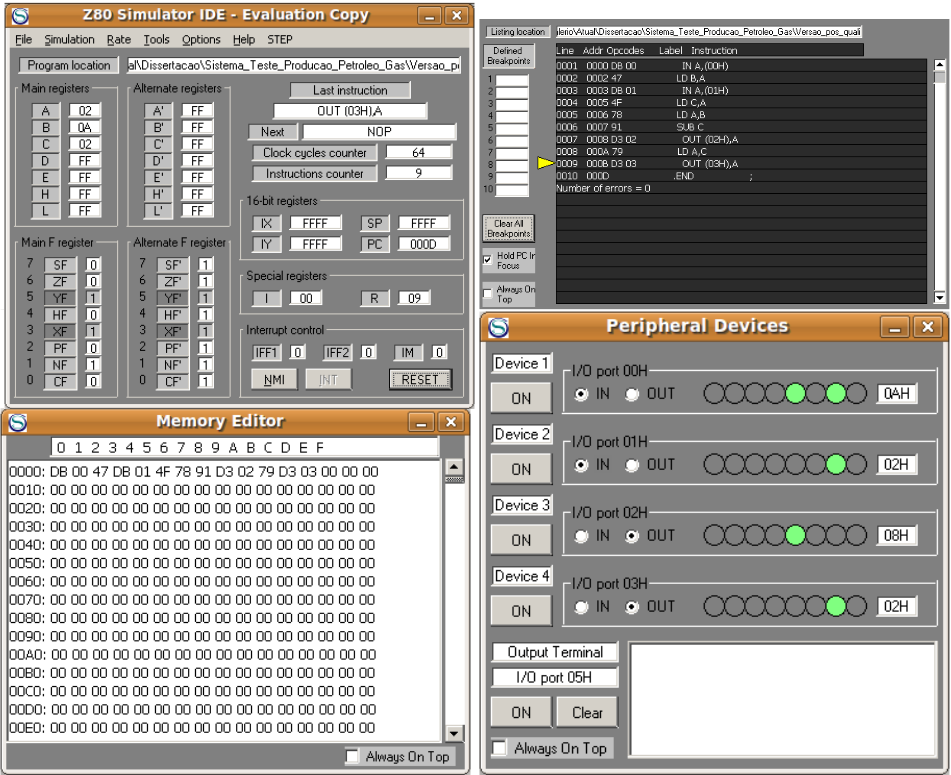
\includegraphics[width=1.0\textwidth]{images/Simulator_Full.png}
%\includegraphics[width=0.45\textwidth]{images/Simulator_Peripheral_Devices.png}
\caption{Window of Z80 simulator \cite{Simulator_z80}.}
\label{fig:simulacao}
\end{figure}



\section{Related work}
\label{sec:relatedworks}

There exists several approaches to model hardware and instruction set
using B a.  The paper \cite{springerlink:Yuan2011} reports a method to
specify, design and construct sound and complete instruction set model
by stepwise refinement and formal proof using Event-B. It also
discusses desirable properties of the instruction set model. However,
our work \cite{Valerio_SBMF09} and \cite{Subotic2010} use the B
method, that seems quite appropriated to software development, because
it has an implementable language defined, called B0, a model-driven
approach \cite{Dantas_SBMF08} to develop software from the functional
specification level down to assembly, and tools to convert the models
to a programming language. 

A related experience on using B in the design of secure
micro-controllers is present in \cite{Marc20113}. It tries to show the
feasibility of such a technique for high confidence trustful
devices. The work \cite{Subotic2010} describes a similar approach with
MIPS CPU architecture and it shows how the CPU is formally specified
and implemented using the B method.

% 
%There are in the literature several
%approaches~\cite{BHDL_2003,DBLP:journals/entcs/EvansG08,DBLP:conf/fmco/Leuschel08,DBLP:conf/asm/Wright08}
%to model hardware and the virtual machines using B. In these works, the B
%has been used successfully to model the operational semantic. However the cost of modeling is still expensive. 
%
%These recent works \cite{Marc20113,springerlink:Yuan2011} have a similar approach using Event B. 
%However, our work use the B method, that seems more appropriated to software development, because it has
%implementable language defined, called B0, and tools to convert the models to a programming language.
%
%
%The main motivation of our research is the development of verified
%software up to the assembly level, which requires specifying the
%semantics of the underlying hardware. Thus some aspects were not
%modeled in our work such as the execution time of the instructions.
%Also we did not consider the micro architecture of the hardware as the scope of
%our work does not include hardware verification. 


 
\section{Conclusions}
\label{sec:conclusions} 

% Um pequeno resumo do trabalho
This work has shown an approach to the formal modeling of the
instruction set of microcontroller using the B method.  During the
construction of this model, some problems were found in the official
reference for Z80 microcontroller~\cite{Z80_manual}. We have consulted
different sources \cite{Simulator_z80,UndocumentedZ80,Z80_manual} to
avoid such problems in modeling and have developed a case study: a
verified embedded software.  This case study was interesting to as a
feasibility analysis of the approach to derive formally assembly code
from a specification of functional requirements in the B method.

%TODO: COLOCAR AQUI OS PRINCIPAIS BENEFÍCIOS PROPORCIONADOS PELO TRABALHO



% fundamenta melhor o trabalho já desenvolvido. Citar o artigo SBMF e a dissertação. 
% Os meus trabalhos já desenvolvidos/ resultados atuais.
The following works are directly related to the objective this paper.
The approach to develop verified software down to the assembly level
using B was described in~\cite{DantasSemish2008}. A first case study
for this approach was reported in~\cite{Dantas_SBMF08}, presenting
more details as well as a small software that developed up to assembly
level in three different platforms. A general view of a previous used
in verification process were presented in~\cite{Valerio_SBMF09}. The
model presented in the current paper added support for animation in
ProB and the representation of external actions (interruptions).
%Link com o parágrafo anterior 
This set of papers present an important step to software verification
up to assembly language, showing the current difficulties and
suggesting improvements in tools supporting the B method.


% [Trabalhos futuros ] LLVM:Existe também a pretensão de especificar as
In the future, we plan to improve the support for the development of
software with the B method from functional specification to assembly
level, using the Z80 model presented in this work. For instance, the
mechanic compilation from B algorithmic constructs to assembly
platform is also envisioned. Finally, another important activity is to
develop a formal model of a platform used in LLVM
Compiler~\cite{DBLP:conf/cgo/LattnerA04}, which would enable us to
integrate different compilation techniques into our B-based framework.



% Conclusão: toque final
%Several iterations were needed to provide the good library definitions as well as
%to fine-tune the model of the microcontroller instructions by factoring common
%functionalities into auxiliary definitions.  

\subsubsection{Acknowledgements:} The animation of the model would not
have been possible without the help of Michael Leuschel who kindly
provided feedback and developed several improvements to ProB to meet our
needs.

% This work was partially supported by INES (www.ines.org.br),
%funded by CNPq grant 573964/2008-4 and by CNPq grants 553597/2008-6, 550946/2007-
%1, and 620132/2008-6

  
%\paragraph{Acknowledges:}
%This work was partially supported by INES (www.ines.org.br), funded by CNPq
%grant \ldots
%573964/2008-4 and by CNPq grants 553597/2008-6, 550946/2007-1, and 620132/2008-6..

%\bibliographystyle{splncs}


\bibliographystyle{plain}
\bibliography{paper}
% [To change the format; to add: thesis suggested by David, Article from ABZ 2010 suggested by David  ]
% \begin{thebibliography}{5}
% 


\end{document}

%
% \bibitem {clar:eke}
% Clarke, F., Ekeland, I.:
% Nonlinear oscillations and
% boundary-value problems for Hamiltonian systems.
% Arch. Rat. Mech. Anal. {\bf 78} (1982) 315--333
% %
% \bibitem {clar:eke:2}
% Clarke, F., Ekeland, I.:
% Solutions p\'{e}riodiques, du
% p\'{e}riode donn\'{e}e, des \'{e}quations hamiltoniennes.
% Note CRAS Paris {\bf 287} (1978) 1013--1015
% %
% \bibitem {mich:tar}
% Michalek, R., Tarantello, G.:
% Subharmonic solutions with prescribed minimal
% period for nonautonomous Hamiltonian systems.
% J. Diff. Eq. {\bf 72} (1988) 28--55
% %
% \bibitem {tar}
% Tarantello, G.:
% Subharmonic solutions for Hamiltonian
% systems via a $\bbbz_{p}$ pseudoindex theory.
% Annali di Matematica Pura (to appear)
% %
% \bibitem {rab}
% Rabinowitz, P.:
% On subharmonic solutions of a Hamiltonian system.
% Comm. Pure Appl. Math. {\bf 33} (1980) 609--633
% \end{thebibliography}
%

